\documentclass[
     11pt,         % font size
     a4paper,      % paper format
     oneside,
     ]{article}

%%%%%%%%%%%%%%%%%%%%%%%%%%%%%%%%%%%%%%%%%%%%%%%%%%%%%%%%%%%%

% PACKAGES:

% Use German :
\usepackage[USenglish]{babel}
% Input encoding
\usepackage[utf8]{inputenc}
% Font encoding
\usepackage[T1]{fontenc}
% Einbinden von URLs:
\usepackage{url}
% hyperrefs in the documents
\usepackage[bookmarks=true,colorlinks,pdfpagelabels,pdfstartview = FitH,bookmarksopen = true,bookmarksnumbered = true,linkcolor = black,plainpages = false,hypertexnames = false,citecolor = black,urlcolor=black]{hyperref} 
%\usepackage{hyperref}
% Include Graphic-files:
\usepackage{graphicx}
% Include PDF links
%\usepackage[pdftex, bookmarks=true]{hyperref}
% Fuer Textsatz
\usepackage{setspace}
% For bibliography style
\usepackage[numbers]{natbib}
% for Latex symbols
\usepackage{doc}
\usepackage[]{algorithm2e}
\usepackage{float}
\usepackage{tikz}
\usetikzlibrary{decorations.markings}
\usepackage{caption}
\usepackage{subcaption}
\usepackage{lipsum}
\usepackage{mwe}
\usepackage{pgfplots}
\usepackage{amsmath}
\usepackage{movie15}
\usepackage{hyperref}
\usepackage{mathtools}
\usepackage{amsthm}
\newtheorem{name}{Printed output}
\newtheorem{mydef}{Definition}
\newtheorem{mytheory}{Theorem}
\newtheorem{myProof}{Proof}
\newcommand{\vect}[1]{\boldsymbol{#1}}

\begin{document}
	\section{Dynamic System}
	\label{sec:DynamicSystem}
	In this chapter, we are introducing concepts of \textit{Dynamic System }, especially those terminologies and concept of \textit{flow}, which is a common kind of dynamic system and our theories of measuring time dependency characteristics is using on flow system. \\
	\subsection{Dynamic System}
	Enormous variety of different kinds of system can be called "dynamic system". Generally, if a system evolves with time, possibly it is one of dynamic systems, and this also predicates the significance of analyzing time dependency property of dynamic system. For instance ,double pendulum which is a pendulum with another pendulum attached to its end can be describe as a dynamic system and exhibits rich dynamical behavior. \\
	
	A dynamic system usually has various \textbf{states} $S_{i}$ at different time. Usually system evolving with time leads a sequence of states $S_{0}$, $S_{1}$,...,$S_{i}$,...,$S_{n-1}$, $S_{n}$, which is called \textbf{trajectory}, and \textbf{state transition} is the system changes from one state to another. Still take the double pendulum as an example, $S_{i}$ is the position of those two pendulums $(x_{1i},y_{1i},x_{2i},y_{2i})$ , where $(x_{1i},y_{1i})$ and $x_{2i},y_{2i})$ are the coordinate position of those two pendulums, while the state from $S_{i}(x_{1i},y_{1i},x_{2i},y_{2i})$ to $S_{j}(x_{1j},y_{1j},x_{2j},y_{2j})$ is a state transition and in a continuity time period all states composed a trajectory as the figure\ref{fig:DoublePendulums}.\\
	\begin{figure}[H]
		\centering
		\includegraphics[width=0.5\textwidth]{pic/DoublePendulums.png}
		\caption{\tiny Double pendulums model trajectory.\cite{DoublePendulum} }
		\label{fig:DoublePendulums}
	\end{figure}
	
	Mathematically, dynamic system can be describe in continuous case by Ordinary differential equations:
	\begin{eqnarray}
		\vect{X}^{'}(t;t_{0},\vect{X}_{0})=\frac{d\vect{X}(t;t_{0},\vect{X}_{0})}{dt}=\vect{V}(\vect{X},t)\\
		\vect{X}(t_{0};t_{0},\vect{X}_{0})=\vect{X}_{0}
	\end{eqnarray}
	where $\vect{X}(t;t_{0},\vect{X}_{0})\in \vect{R^{n}}$, $t\in R$,$\vect{V}:\vect{R^{n}}\rightarrow\vect{R^{n}}$, $t_{0}$ is initial time and $\vect{X_{0}}$ is initial state at $t_{0}$.\\
	The solution of equation $\psi(t,t_{0}\vect{X_{0}})$ is the trajectory of the dynamic system.\\
	In discrete case, equations:
	\begin{eqnarray}
		\Delta\vect{X}(t;t_{0},\vect{X}_{0})=\vect{X}(t+1;t_{0},\vect{X}_{0})-\vect{X}(t;t_{0},\vect{X}_{0})=\vect{V}(\vect{X},t)\\
		\vect{X}(t_{0};t_{0},\vect{X}_{0})=\vect{X}_{0}
	\end{eqnarray}
	where $t\in Z$. In dynamical system visualization area, usually the discrete equations are applied, which will mainly occur in next parts of this thesis.\\
	It is also possible to use other equations to exhibit the dynamic system, for instance, $\vect{X}(t+1,t_{0},\vect{X}_{0})=V(\vect{X}(t,t_{0},\vect{X}_{0}))$. If $V(\vect{X}(t,t_{0},\vect{X}_{0}))$ depends on $t$, then the system is time-dependent, or it is time-independent also called stationary system.
	
	\subsection{Fluid Flow And Vector Field}
	As one of the most important dynamical system, fluid flow is fluids such as gas and liquids in motion. The intuitive example of fluid flow is air flow which is wind around us. Obviously, it is possible to measure numerous properties of the fluid flow, for example velocity, temperature and stress. In my thesis, I focus on the variable-velocity in 2 dimension.\\
	As to velocity, it is common to assign a vector $\vect{V}\in \vect{R^{n}}$ to present a velocity. The magnitude of vector $\lvert\vect{V}\rvert=\sqrt{\sum_{i=0}^{i=n-1}v_{i}^{2}}$ is the magnitude of the velocity and $v_{i}$ is the magnitude in one dimension. Vectors presenting velocity at points in fluid flow compose the vector field of the fluid flow. In this thesis, I am using 3d vector data in 3d domain to present data time dependent in a fluid flow. For more specific, we measure the velocity 401 times in the same 2d space in a period which is 10 seconds, so that we get the velocity of fluid flow during in the area during this 10 seconds period. Afterwards, build a 3 dimension data domain, where two dimensions present the 2d space and other dimension presents time. \\
	In vector field visualization, it is quite popular to present a vector by arrow, the length of the arrow standing for the magnitude of velocity and the direction of arrow presenting direction.

	\begin{figure}[H]
		\begin{minipage}{0.5\textwidth}
			\centering
			\includegraphics[width=0.5\textwidth]{pic/DataModel.png}
			\caption{\tiny Data: x axis and y axis present the space, z axis present time. And two slices at time 5.0s and 7.5s}
			\label{fig:DataModel}
		\end{minipage}
		\begin{minipage}{0.5\textwidth}
			\centering
			\includegraphics[width=0.5\textwidth]{pic/VelocityDataAt7dot5s.png}
			\caption{\tiny Velocity of the space at time=7.5s}
			\label{fig:VelocityDataAt7.5s}
		\end{minipage}
	\end{figure}	
	Mathematically, as similar as dynamic system:\\
	Define a 2d space $\vect{D}$,  $\vect{D}\subset \vect{R}^{2}$, $\vect{X}\in \vect{D}$.\\
	Define a 3d data domain $\vect{\Omega}$, $\vect{\Omega} \subset \vect{R}^{2}\times\vect{R}$, where 2 dimensions are space and 1 dimension is time. $\vect{\xi}(\vect{X},T) \in \vect{\Omega}$ means $\vect{X}$ at time $T$.To be specific, $\vect{V}\subset \Omega$ but with the third dimension fixed, only consider about 2 dimensions of the vector data set.\\
	Define a 2d vector data set $\vect{V}(\xi(\vect{X},T))$ is the velocity at position $\vect{X}(x,y) \in D$ at time $T$ and $\vect{V}$ satisfied Lipschitz continuous.\\
	Here Lipschitz continuous means:\\
	$\forall\vect{X_{01}}, \vect{X_{02}}\in \vect{D}$ and $\forall t\in R$, $\exists\geq0$ such that:\\
	$$\lVert \vect{V}(t;\xi(\vect{X_{01}},T+t))-\vect{V}(t;\xi(\vect{X_{01}},T+t))\rVert\leq K\lVert\vect{X_{01}}-\vect{X_{02}}\rVert$$

	And flow can be describe by below equations:\\
	\begin{eqnarray}
	\vect{\xi}^{'}(t;\xi(\vect{X_{0}},T+t))=\frac{\vect{\xi}(t;\xi(\vect{X_{0}},T+t))}{dt}=\vect{V}(t;\xi(\vect{X_{0}},T+t))\\
	\vect{\xi}(0;\vect{X}_{0},T)=\xi(\vect{X_{0}},T)
	\end{eqnarray}
	In discrete case, equations:
	\begin{eqnarray}
	\Delta\vect{X}(t;t_{0},\xi(\vect{X}_{0},T+t))=\vect{X}(t+1;t_{0},\xi(\vect{X}_{0},T+t))-\vect{X}(t;t_{0},\xi(\vect{X}_{0},T+t))\\
	\Delta\vect{X}(t;t_{0},\xi(\vect{X}_{0},T+t))=\vect{V}(t;\xi(\vect{X_{0}},T+t))\\
	\vect{\xi}(0;\vect{X}_{0},T)=\xi(\vect{X_{0}},T)
	\end{eqnarray}
	where $t, T\in Z$. 

	Figure\ref{fig:DataModel} and figure\ref{fig:VelocityDataAt7.5s} show outline of the data and velocity vectors at time=7.5s.\\
	So far, it only shows vector field itself, but does not show how vectors changing in the period. In paraview, making a video of the vector field alternatively can show vector altering. The idea is getting a series of picture which present the velocity at one moment and take one picture as a frame of the video.By the velocity video, people can get the rough idea of velocity changing.\\
	However, it is still not a good way to show the time dependency, because there is not specific quantitative measurement to present the property directly. 
	
	\section{Stream Line and Path Line}
	\label{sec:Streamline and pathline}
	\subsection{Stream  Line}
	Streamlines are a family of curves that are instantaneously tangent to the velocity vector of the flow. These show the direction in which a massless fluid element will travel at any point in time\cite{StreamlineDefine}. This denotes that streamlines indicate velocity at one specific moment and presenting the vector structure at this moment. Actually, a streamline is the path traced out by a massless particle as it moves with the flow at this moment.\\
	Moreover, stream line is a restrict Eulerian approach which is used to obtain a clear idea of the flow at one particular instant. People can take it as a photograph of the flow, for instance in the vector field we mentioned before(see figure\ref{fig:DataModel}), every $Z$ direction slice is a Eulerian approach view.\\
	When construct the streamline, we set a "virtual time step" $\Delta t$, which means it is only used to computing points along the streamline. In discrete case, pick a point call seed from the space with velocity vector $V$ and get the next point of the streamline by $V\cdot\Delta t$, then repeat from this point until to the total time $t_{n}$. Even though, time is mentioned frequently when construct stream line, actually it does not related to real time, so stream line is time-independent.\\
	Mathematically, define $\phi^{t}(\vect{X}_{0},T)\in D$ as the point streamline reaching at time $t$ after start, and the streamline starts at seed $\xi(\vect{X_{0}},T)$. \\
	Satisfied differential equations:\\
	\begin{eqnarray}
	\frac{d\phi^{t}(\vect{X}_{0},T)}{dt}=V(\phi^{t}(\vect{X}_{0},T),T)\\
	phi^{t=0}(\vect{X}_{0},T)=\xi(\vect{X_{0}},T)
	\label{equation:Streamline1}
	\phi^{t=0}(\vect{X}_{0},T)=\xi(\vect{X_{0}},T)
	\label{equation:Streamline2}
	\end{eqnarray}
	where $t,T\in R$.\\
	In discrete case, equations:\\
	\begin{eqnarray}
	\lVert\phi^{t+1}(\vect{X}_{0},T)-\phi^{t}(\vect{X}_{0},T)\rVert=V(\phi^{t}(\vect{X}_{0},T),T)\\
	\phi^{t=0}(\vect{X}_{0},T)=\xi(\vect{X_{0}},T)
	\end{eqnarray}
	where $t,T\in Z$.\\ 
	Below is the algorithm when construct stream lines.\\
	\begin{algorithm}[H]
		\KwData{Vector field data set}
		\KwResult{stream lines}
		Set the time slice where stream lines would be.\\
		Select space area which seeds from and the number of seeds$s$.\\
		Get seeds by picking points uniform from the area or using Poisson sampling.\\ 
		Set time step $\Delta t$ and total time $t_{n}$. \\
		Get number of points along one stream line $n$.\\
		\For {$i\leftarrow 0$ \KwTo $s-1$}
		{
			Set seed coordinate $S_{i0}$\\
			\For{$j\leftarrow 0$ \KwTo $n-1$}{
				Get velocity $V_{ij}$ of the seed by Runge-Kutta 4th order interplation.\\
				Computing the next point $S_{ij+1}$ coordinate by $S_{ij}+V\cdot \Delta t$;\\
				use a vtk line to contact the $S_{ij+1}$ and $S_{ij}$\\
				}
			Show one stream line;
			}
	\end{algorithm}
    In the figure\ref{fig:streamlineattime=5s}, we can see some stream lines structure. Some stream lines are closed, which means at this time slice flow is an vortex.
	\begin{figure}[H]
	\centering
	\includegraphics[width=0.8\textwidth]{pic/streamlineattime=5s.png}
	\caption{{\tiny some streamlines at time=5s. Arrows are the flow and those tubes are streamlines}}
	\label{fig:streamlineattime=5s}
	\end{figure}
	
	\subsection{Path Line}
	Except Eulerian approach (also called Eulerian way), \textit{Lagrangian way} is the approach tracking individual massless fluid particles in flow during a period of time in a vector field. Unlike Eulerian approach which defines a control volume and describes the vector field in it at one specific time.\\
	Path lines is exactly curves reflecting Lagrangian way. Path lines are trajectories that individual massless fluid particles flow, which can be thought of as "recording" the path of a fluid element in the flow over a certain period. The direction path lines take will be determined by the stream lines of the fluid at each moment in time\cite{PathlineDefine}. Basing on definitions, the main difference between path lines and stream lines is related to time, i.e stream lines are time-independent while path lines are time-independent. Exactly because of this property, I will compare stream lines and path lines in next chapters and show how the vector field data dependent on time.\\
	When construct path lines, we pick some seeds where path lines start at one moment $T_{0}$. As similar as constructing stream lines, the "time step" $\Delta t$ should also be set, which is "real time" here. In other words, when compute the $n^{th}$ point of path line after the $(n-1)^{th}$ point, the velocity at time $T_{0}+n\cdot\Delta t$ is applied.\\
	 \begin{figure}[H]
	 	\begin{subfigure}{0.45\textwidth}
	 		\centering
	 		\includegraphics[width=0.7\textwidth]{pic/ConstructStreamlineAndPathlinet0t1.png}
	 		\caption{{\tiny velocity at time $t_{0}$ and $t_{1}$ of a simple vector field data.}}
	 		\label{fig:ConstructStreamlineAndPathlinet0t1}
	 	\end{subfigure}
	 	\begin{subfigure}{0.45\textwidth}
	         \centering
	 		 \includegraphics[width=0.7\textwidth]{pic/ConstructStreamlineAndPathlinet2t3.png}
	 		 \caption{{\tiny velocity at time $t_{2}$ and $t_{3}$ of a simple vector field data.}}
	 		 \label{fig:ConstructStreamlineAndPathlinet2t3}
	 	\end{subfigure}
	 	\begin{subfigure}{0.45\textwidth}
	 		 \centering
	 		 \includegraphics[width=0.7\textwidth]{pic/pathline.png}
	 		 \caption{{\tiny path line in period $t_{0}$ to $t_{3}$.}}
	 		 \label{fig:pathline}
	 	\end{subfigure}
	 	\begin{subfigure}{0.45\textwidth}
	    	 \centering
	 		 \includegraphics[width=0.7\textwidth]{pic/streamline.png}
	 		 \caption{{\tiny streamline at time $t_{3}$.}}
	 		 \label{fig:streamline}
	 \end{subfigure}
	 \caption{{\tiny Simple example of stream line and path line.}}
	 \label{fig:streamlineandpathline}
	 \end{figure}
	\begin{figure}[H]
			\centering
			\includegraphics[width=0.35\textwidth]{pic/pathlines.png}
			\caption{{\tiny some pathlines at time=5s and end at 8s from those red seeds. we can see pathline go through the flow through time.}}
			\label{fig:pathlineatfrom5s}
		\end{figure}
	Mathematically define $\psi^{t}(X_{0},T)\in\vect{D}$ is the path line point after time $t$ start from $\vect{X}_{0}$ at $T$, $t,T\in R$.\\
	And pathline is the solution of differential equations:\\
    \begin{eqnarray}
    \frac{d\psi^{t}(\vect{X}_{0},T)}{dt}=V(\psi^{t}(\vect{X}_{0},T),T+t)\\
    \psi^{t=0}(\vect{X}_{0},T)=\xi(\vect{X_{0}},T)
    \end{eqnarray}
    In discrete case, equations:\\
    \begin{eqnarray}
    \lVert\psi^{t+1}(\vect{X}_{0},T)-\psi^{t}(\vect{X}_{0},T)\rVert=V(\psi^{t}(\vect{X}_{0},T),T+t)\\
    \phi^{t=0}(\vect{X}_{0},T)=\xi(\vect{X_{0}},T)
    \end{eqnarray}
    where $t,T\in Z$.\\ 
    Apparently, equations described stream lines and path lines indicate path lines are time-dependent and stream lines are not.\\
	Moreover, as stream lines and path lines are continuous and steady by given a vector field data set, which means if set a massless fluid particle in any point along the stream line or path line curve,by controlling the time the particle flow, the exactly overlapped stream line and path line can be constructed . As this theory existing, we can know time dependency analysis basing on comparison of path line and stream line is steady.\\
	Mathematically, it is shown:\\
	\begin{eqnarray}
	\phi^{t_{m}+t_{n}}(\vect{X}_{0},T)=\phi^{t_{n}}(\phi^{t_{m}}(\vect{X}_{0},T),T+t_{m})=\phi^{t_{m}}(\phi^{t_{n}}(\vect{X}_{0},T),T+t_{n})
	\label{Equation:StreamlinePoint}
	\end{eqnarray}
	\begin{eqnarray}
	\psi^{t_{m}+t_{n}}(\vect{X}_{0},T)=\psi^{t_{n}}(\psi^{t_{m}}(\vect{X}_{0},T),T+t_{m})=\psi^{t_{m}}(\psi^{t_{n}}(\vect{X}_{0},T),T+t_{n})
	\end{eqnarray}
	where $T,t_{m},t_{n}\in R$.
    \section{Topology Based on Stream Lines and Path Lines}
    \label{sec:Topology}
	\section{Distance of Streamline and Pathline}
	\label{sec:Distance}
    As we mentioned in section of stream line and path line, we define $\phi^{t}(\vect{X}_{0},T)$ as the point stream line starting at seed $\vect{X}_{0}$ and time $T$ reaching after "virtual time" $t$ and $\psi^{t}(\vect{X}_{0},T)$ as the point stream line starting at seed $\vect{X}_{0}$ and time $T$ reaching after "true time" $t$. If we set the "virtual time " equal to the "real time", time-dependency property of vector field data along the stream line and path line starting at the same seed can be analyzed, as stream line is time-independent and path line is time independent.\\
    Analogously to  other scientific analysis, keeping other variables holding and only concern the control variable, here maintain "virtual time" equal to "real time", and only analyze the vector change along stream lines and path lines starting at different seeds in the time period, which is time-dependency property of vector along path lines and stream lines.\\
    For measuring time-dependency, we introduce a concept \textit{Distance of Stream Line and Path Line starting at $\vect{X}_{0}$ and time $T$ after time $t$}, for short call it $SPD_{t}$.\\
    \subsection{Definition}
    \begin{mydef}
	\textbf{\textit{Distance of Stream Line and Path Line starting at $\vect{X}_{0}$ and time $T$ after time $t$}} (\textbf{\textit{$SPD_{t}$}}) is the distance of two points stream line and path line which start at $\vect{X}_{0}$ and time $T$ after time $t$ reaching. Mathematically, it is marked as $SPD(\vect{X}_{0},T,t)$.\\
    \end{mydef}
    Mathematically, $SPD(\vect{X}_{0},T,t)$ defined as below:
	\begin{eqnarray}
	\label{Equation:SPDDef}
	SPD(\vect{X}_{0},T,t)=\biggr\lVert\phi^{t}(\vect{X}_{0},T)-\psi^{t}(\vect{X}_{0},T+t)\biggr\rVert\\
	SPD(\vect{X}_{0},T,t)=\biggr\lVert\int_{\tau=0}^{\tau=t}\biggr( V(\phi^{\tau}(\vect{X}_{0},T),T)-V(\psi^{\tau}(\vect{X}_{0},T),T+\tau)\biggr) d\tau\biggr\rVert
	\end{eqnarray}
	The discrete case:
	\begin{eqnarray}
		\label{Equation:SPD}
		SPD(\vect{X}_{0},T,t)=\biggr\lVert\sum_{i=0}^{i=n}\biggr( V(\phi^{t_{i}}(\vect{X}_{0},T),T)-V(\psi^{t_{i}}(\vect{X}_{0},T),T+t_{i})\biggr)\cdot\Delta t_{i}\biggr\rVert
	\end{eqnarray}
	where $t_{n}=t, t_{0}=0$ and the time sequence  $t_{0},t_{1},...,t_{i},...,t_{n} $ and $\Delta t_{i}=t_{i}-t_{i-1}$.\\
	Here is the proof for equation\ref{Equation:SPD}
	\begin{myProof}
		As equation\ref{Equation:StreamlinePoint}:\\
		$\phi^{t_{1}}(\vect{X}_{0},T)=\vect{X}_{0}+\Delta t_{1}\cdot V(\vect{X}_{0},T);$\\
		\\
		$\phi^{t_{2}}(\phi^{t_{1}}(\vect{X}_{0},T),T)$\\
		$=\phi^{t_{1}}(\vect{X}_{0},T)+\Delta t_{2}\cdot V(\phi^{t_{1}}(\vect{X}_{0},T),T)$\\
		$=\vect{X}_{0}+\Delta t_{1}\cdot V(\vect{X}_{0},T)+\Delta t_{2}\cdot V(\phi^{ t_{1}}(\vect{X}_{0},T),T);$\\
		$$...$$
		$\phi^{ t_{i}}(\phi^{ t_{i-1}}(\vect{X}_{0},T),T)$\\
		$=\phi^{ t_{i-1}}(\vect{X}_{0},T)+\Delta t_{i}\cdot V(\phi^{ t_{i-1}}(\vect{X}_{0},T),T)$\\
		$=\vect{X}_{0}+\Delta t_{1}\cdot V(\vect{X}_{0},T)+...+\Delta t_{i-1}\cdot V(\vect{X}_{0},T)+\Delta t_{i}\cdot V(\phi^{ t_{i-1}}(\vect{X}_{0},T),T);$\\
		$$...$$
		$\phi^{\Delta t_{n}}(\phi^{ t_{n-1}}(\vect{X}_{0},T),T)$\\
		$=\phi^{ t_{n-1}}(\vect{X}_{0},T)+\Delta t_{n}\cdot V(\phi^{ t_{n-1}}(\vect{X}_{0},T),T)$\\
		$=\vect{X}_{0}+\Delta t_{1}\cdot V(\vect{X}_{0},T)+...+\Delta t_{n-1}\cdot V(\vect{X}_{0},T)+\Delta t_{n}\cdot V(\phi^{t_{n-1}}(\vect{X}_{0},T),T)$;\\
		\\
		$\phi^{t}(\vect{X}_{0},T)=\phi^{\Delta t_{n}}(\phi^{t_{n-1}}(\vect{X}_{0},T),T)$\\
		\\
		As similar to $\phi^{t}(\vect{X}_{0},T)$, we have $\psi^{t}(\vect{X}_{0},T+t)$:\\
		\\
		$\psi^{\Delta t_{n}}(\psi^{t_{n-1}}(\vect{X}_{0},T+t_{n-1}),T)$\\
		$=\psi^{ t_{n-1}}(\vect{X}_{0},T+t_{n-2})+\Delta t_{n}\cdot V(\psi^{t_{n-1}}(\vect{X}_{0},T),T+t_{n-1})$\\
		$=\vect{X}_{0}+\Delta t_{1}\cdot V(\vect{X}_{0},T+t_{1})+...+\Delta t_{n-1}\cdot V(\vect{X}_{0},T+t_{n-2})+\Delta t_{n}\cdot V(\psi^{ t_{n-1}}(\vect{X}_{0},T),T+t_{n-1});$\\
		\\
		$\psi^{t}(\vect{X}_{0},T)=\psi^{\Delta t_{n}}(\phi^{t_{n-1}}(\vect{X}_{0},T),T)$\\
		\\
		So basic on equation\ref{Equation:SPDDef}
		$SPD(\vect{X}_{0},T,t)=\biggr\lVert\phi^{t}(\vect{X}_{0},T)-\psi^{t}(\vect{X}_{0},T+t)\biggr\rVert$\\
		$=\biggr\lVert (\vect{X}_{0}+\Delta t_{1}\cdot V(\vect{X}_{0},T)+...+\Delta t_{n-1}\cdot V(\vect{X}_{0},T)+\Delta t_{n}\cdot V(\phi^{t_{n-1}}(\vect{X}_{0},T),T))-(\vect{X}_{0}+\Delta t_{1}\cdot V(\vect{X}_{0},T+t_{1})+...+\Delta t_{n-1}\cdot V(\vect{X}_{0},T+t_{n-2})+\Delta t_{n}\cdot V(\psi^{t_{n-1}}(\vect{X}_{0},T),T+t_{n-1}))\biggr\rVert$\\
		$=\biggr\lVert\sum_{i=0}^{i=n}\biggr( V(\phi^{t_{i}}(\vect{X}_{0}),T)-V(\psi^{t_{i}}(\vect{X}_{0}),T+t_{i})\biggr)\cdot\Delta t_{i}\biggr\rVert$
		
		
		
	\end{myProof}
	
	Furthermore, if both of the "virtual time" of stream line and "real time" of path line are set as $t_{n}$ , call $t_{n}$ \textit{end time} and points stream line and path line reaching at end time \textit{end points}.
	\begin{mydef}
		\textbf{\textit{Distance of Stream Line and Path Line starting at $\vect{X}_{0}$ and time $T$}} (\textbf{\textit{$SPD_{t_{n}}$}}) is the distance of end points stream line and path line which start at $\vect{X}_{0}$ and time $T$. Mathematically, it is marked as $SPD(\vect{X}_{0},T,t_{n})$.\\
	\end{mydef}
	\begin{eqnarray}
	SPD(\vect{X}_{0},T,t_{n})=\biggr\lVert\phi^{t_{n}}(\vect{X}_{0},T)-\psi^{t_{n}}(\vect{X}_{0},T)\biggr\rVert\\
	SPD(\vect{X}_{0},T,t_{n})=\biggr\lVert\int_{\tau=0}^{\tau=t_{n}}\biggr( V(\phi^{\tau}(\vect{X}_{0}),T)-V(\psi^{\tau}(\vect{X}_{0}),T+\tau)\biggr) d\tau\biggr\rVert
	\label{equation:SPD}
	\end{eqnarray}
	\begin{figure}[H]
		\centering
		\includegraphics[width=0.65\textwidth]{pic/tu1.pdf}
		\caption{\tiny Definition of $SPD$ }
		\label{fig:SPD}
	\end{figure}
	Just as the equation \ref{equation:SPD} shown, $SPD(\vect{X}_{0},T,t_{n})$ is magnitude of integration of $\Delta V_{\tau}=V(\phi^{\tau}(\vect{X}_{0},T),T)-V(\psi^{\tau}(\vect{X}_{0},T),T+\tau)$  along the stream line and path line, which means it weights vector change along the stream line and path line at time period $t_{n}$ after start time $T$ and this is vector field time dependency. It is easy to learn that $SPD(\vect{X}_{0},T,t_{n})$ depends on $\vect{X}_{0}$,$T$ and $t_{n}$. As it is mentioned before $t_{n}$ is set, so $T$ and $X_{0}$ can be modified , which leads two cases to compare vector time dependency in the data domain.\\
	\subsection{Theorem}
	\textbf{Case One:} Hold $T$, compare $SPD(\vect{X}_{0i},T,t_{n}), \vect{X}_{i0}\in\vect{D}$ of different seeds $\vect{X}_{0i}$.\\
	\textbf{Case Two:} Hold $\vect{X}_{0}$, compare $SPD(\vect{X}_{0},T_{i},t_{n}), T_{i}\in R$ of different start time $T_{i}$.\\
	As the simple example shown in figure\ref{fig:SPDCompare}, vectors the left part of in the domain changed faster than the right part. Picture g indicates $SPD_{t_{5}}$ in left is greater than in right, while picture h indicates $SPD_{t_{5}}$ starting at time $t_{1}$ is greater than starting at time $t_{0}$.\\
	
	\begin{figure}[H]
		\begin{subfigure}{0.3\textwidth}
			\centering
			\includegraphics[width=0.7\textwidth]{pic/SPD/1.pdf}
			\caption{{\tiny velocity at time $T_{0}$ of a simple vector field data.}}
			\label{fig:SPDT0}
		\end{subfigure}
		\begin{subfigure}{0.3\textwidth}
			\centering
			\includegraphics[width=0.7\textwidth]{pic/SPD/2.pdf}
			\caption{{\tiny velocity at time $T_{1}$ of a simple vector field data.}}
			\label{fig:SPDT1}
		\end{subfigure}
		\begin{subfigure}{0.3\textwidth}
			\centering
			\includegraphics[width=0.7\textwidth]{pic/SPD/3.pdf}
			\caption{{\tiny velocity at time $T_{2}$ of a simple vector field data.}}
			\label{fig:SPDT2}
		\end{subfigure}
		\begin{subfigure}{0.3\textwidth}
		    \centering
			\includegraphics[width=0.7\textwidth]{pic/SPD/4.pdf}
			\caption{{\tiny velocity at time $T_{3}$ of a simple vector field data.}}
			\label{fig:SPDT3}
		\end{subfigure}
		\begin{subfigure}{0.3\textwidth}
			\centering
			\includegraphics[width=0.7\textwidth]{pic/SPD/5.pdf}
			\caption{{\tiny velocity at time $T_{4}$ of a simple vector field data.}}
			\label{fig:SPDT4}
		\end{subfigure}
		\begin{subfigure}{0.3\textwidth}
			\centering
			\includegraphics[width=0.7\textwidth]{pic/SPD/6.pdf}
			\caption{{\tiny velocity at time $T_{5}$ of a simple vector field data.}}
			\label{fig:SPDT5}
		\end{subfigure}
		\begin{subfigure}{0.45\textwidth}
			\centering
			\includegraphics[width=0.7\textwidth]{pic/SPD/7.pdf}
			\caption{{\tiny Case One: set $t_{n}=t_{5}$, stream lines and path lines starting at different seeds and time $t_{0}$.}}
			\label{fig:differentseeds}
		\end{subfigure}
		\begin{subfigure}{0.45\textwidth}
			\centering
			\includegraphics[width=0.7\textwidth]{pic/SPD/8.pdf}
			\caption{{\tiny Case Two: set $t_{n}=t_{5}$, stream lines and path lines starting at same seeds and different time $T_{0}$ and $T_{1}$.}}
			\label{fig:differenttime}
		\end{subfigure}
		\caption{{\tiny Simple example of $SPD$ of two cases .}}
		\label{fig:SPDCompare}
	\end{figure}
    \begin{mytheory}
    	Apply $SPD(\vect{X}_{0},T,t_{n})$ to visual time-dependency of vector field data set along stream lines and path lines. In those two cases mentioned, $SPD(\vect{X}_{0},T,t_{n})$ is greater, the vector data along stream line and path line is more time-dependent , if $SPD(\vect{X}_{0},T,\tau)$,$\tau in [0, t_{n}]$ is almost monotonous increasing. 
    	\label{Theo:SPD}
    \end{mytheory}
    \subsection{Theorem Analysis}
    As mentioned before, $SPD(\vect{X}_{0},T,t_{n})$ accumulates $\Delta V_{\tau}=V(\phi^{\tau}(\vect{X}_{0},T),T)-V(\psi^{\tau}(\vect{X}_{0},T),T+\tau), \tau\in[0,t_{n}]$ along stream lines and path lines. This idea is very intuitive and simple and most importantly it gives an quantitative measurement to weight time-dependency of vector field data set, which is entirely different from the topology methods.\\
    Nevertheless, utilize of this theorem is limited, because of reason below:
    \begin{itemize}
    	\item First of all, the value of $SPD_{t_{n}}$ depends on the magnitude of the vector strongly.\\ 
    	This implies that if the magnitude of vectors along stream line or path line is great enough, even without highly time-dependent property of the data  $SPD_{t_{n}}$ could be large. Because of this, $SPD_{t_{n}}$ can underestimate or overestimate the time-dependency of vector field.\\
    	Below, give a simple example of stream lines and path lines to show this.\\
    	\begin{figure}[H]
    		\centering
    		\includegraphics[width=0.7\textwidth]{pic/tu4.pdf}
    		\caption{\tiny The left case shows small $SPD_{t_{n}}$ with high time dependency velocity data, while the right case shows greater $SPD_{t_{n}}$ with lower time dependency velocity data along the streamline and pathline.}
    		\label{fig:NorSPD}
    	\end{figure}
    	In the figure\ref{fig:NorSPD}, set time $t_{n}$ and two pairs of stream line and path line start at different seeds and identical start time $T$ . As the length of stream line and path line at left is much smaller than at right, it is easy to say the magnitude of vectors along stream line and path line at right is much greater. However, as both of stream lines maintain almost identical tendency, in addition, path line at left presents more time-dependency property than right. Besides, it is  apparent that $SPD_{t_{n}}$ of the right side is greater than the left side, which is not precise probably.
    	\item Secondly, the value of $SPD_{t_{n}}$ is not accurate, when $SPD(\vect{X}_{0},T,\tau)$,$\tau in [0, t_{n}]$ is not almost monotonous increasing.\\
    	As we mentioned in Theorem 1, the condition of this theorem is $SPD(\vect{X}_{0},T,\tau)$,$\tau in [0, t_{n}]$ is almost monotonous increasing.Mathematically, $	SPD(\vect{X}_{0},T,t_{n})=\biggr\lVert\int_{\tau=0}^{\tau=t_{n}}\biggr( V(\phi^{\tau}(\vect{X}_{0}),T)-V(\psi^{\tau}(\vect{X}_{0}),T+\tau)\biggr) d\tau\biggr\rVert$, and define $\Delta V_{\tau}=V(\phi^{\tau}(\vect{X}_{0},T),T)-V(\psi^{\tau}(\vect{X}_{0},T),T+\tau)$, therefore basically $SPD(\vect{X}_{0},T,t_{n})$ sums up $\Delta V_{\tau},\tau\in[0,t_{n}]$ and get the magnitude of the summing. However, $\Delta V_{\tau},\tau\in[0,t_{n}]$ can be positive and negative. Therefore, when summing up $\Delta V_{\tau},\tau\in[0,t_{n}]$, the negative $\Delta V_{\tau_{1}}, \tau_{1}\in[0,t_{n}]$ can cancel out the positive $\Delta V_{\tau_{2}}, \tau_{2}\in[0,t_{n}]$, which leads underestimation of time-dependency property of vector field.\\
    	\begin{figure}[H]
    		\begin{subfigure}{0.45\textwidth}
    			\centering
    			\includegraphics[width=1\textwidth]{pic/SPD/pathstreamDiff.pdf}
    			\caption{$SPD(\vect{X}_{0},T,\tau), \tau\in[0,t_{n}]$ is not monotonous .}
    			\label{fig:fluctuationSPD}
    		\end{subfigure}
    		\begin{subfigure}{0.45\textwidth}
    			\centering
    			\includegraphics[width=1\textwidth]{pic/SPD/pathstreamdiff2.pdf}
    			\caption{ $SPD(\vect{X}_{0},T,\tau), \tau\in[0,t_{n}]$ is  monotonous.}
    			\label{fig:monotonousSPD}
    		\end{subfigure}
    			\caption{{\tiny figure (a) shows the $SPD(\vect{X}_{0},T,\tau), \tau\in[0,t_{n}]$ is fluctuation and figure (b) shows $SPD(\vect{X}_{0},T,\tau), \tau\in[0,t_{n}]$ is monotonous increasing.}}
    			\label{fig:SPDfluctuationCompare}
    	\end{figure}
    	Comparing figure\ref{fig:SPDfluctuationCompare} (a) and (b), obviously vectors along the stream line and path line in (a) is more strongly time-dependent with a much smaller $SPD_{t_{n}}$, which is unreasonable. If we compare the direction of vectors along the path line and stream line, we can found in (b), the $\Delta V_{\tau},\tau\in[0,t_{n}]$ almost has identical direction, while in (a) the direction of $\Delta V_{\tau},\tau\in[0,t_{n}]$ changes frequency.\\
    	Except the simple example shown, there exist numerous cases of stream line and path line that $SPD(\vect{X}_{0},T,\tau), \tau\in[0,t_{n}]$ fluctuate strongly. In all those case $SPD(\vect{X}_{0},T,t_{n})$ is an inappropriate measurement to gauge time-dependency of vector field data.
    	\item Thirdly, $SPD(\vect{X}_{0},T,t_{n})$ and $SPD(\vect{X}_{0},T,t_{m})$ is not comparable.\\
    	Even in $SPD(\vect{X}_{0},T,\tau), \tau\in[0,max(t_{m},t_{n})]$ monotonous increasing, they are not comparable and the reason is obvious. In this case, a longer period can generate relatively greater value.\\
    	Especially, if the vector field with a vortex which is very common in a flow, the value of $SPD(\vect{X}_{0},T,t_{n})$ will be very dependent on $t_{n}$.
    	\begin{figure}[H]
    		\begin{subfigure}{0.45\textwidth}
    			\centering
    			\includegraphics[width=0.8\textwidth]{pic/SumSPDist=1s.png}
    			\caption{\tiny a pair of stream line and path line start at point $A(x_{0}, y_{0})$ and time T in a vortex, $t_{n}=1s$. streamline is the short one and path line is the long one. }
    		\end{subfigure}
    		\begin{subfigure}{0.8\textwidth}
    			\centering
    			\includegraphics[width=0.45\textwidth]{pic/SumSPDist=2s.png}
    			\caption{\tiny a pair of stream line and path line start at same point $A(x_{0}, y_{0})$ and same time T in a vortex, $t_{m}=2s$.streamline is the short one and path line is the long one.  }
    		\end{subfigure}
    		\caption{a special case of stream line and path line in a vortex.}
    		\label{fig:vortexstreamlineandpathline}
    	\end{figure}
    	In the figure\ref{fig:vortexstreamlineandpathline}, $SPD(\vect{X}_{0},T,t_{n}=1s)$ is greater than $SPD(\vect{X}_{0},T,t_{m}=2s)$ which is unreasonable.This result is because of in the vortex path line and stream line are cycles, the $SPD$ becomes dependent on $t_{n}$, even those in different period time-dependency of data is similar.
    \end{itemize} 
    \subsection{Conclusion}
    Generally,$SPD_{t_{n}}$ only cares about what happens at the final moment and measures time-dependency by this, which means time dependency characteristics is weighted only base on the final result without caring about different situations during $\tau \in(0,t_{n})$.\\
    Although, there are numerous cases where $SPD_{t_{n}}$ can not survey or gauge time dependency characteristics of vector field data set precisely according to those disadvantages mentioned in the last section. Nevertheless, it can reveal the rough idea of time-dependency of vector field. Especially, if along the streamline and pathline $SPD_{\tau}, \tau \in [0,t_{n}]$ almost keep increasing and magnitude of data set do not have huge difference, $SPD_{t_{n}}$ is a good method to measure time-dependency of data.However,if $SPD_{\tau}, \tau \in [0,t_{n}]$, is not almost monotonous but with huge fluctuation, then $SPDis_{t_{n}}$ could not be a good way to measure time dependency property.\\
    At last, most importantly, $SPD_{t_{n}}$ predicates one concept to show time dependency quantitatively and this is the basement concept of those techniques.
    Here we show results of applying $SPD_{t_{n}}$ on the data I mentioned (see figure \ref{fig:DataModel}).
    \begin{figure}[H]
        \begin{subfigure}{0.65\textwidth}
        	\centering
        	\includegraphics[width=1\textwidth]{pic/SPDResulttime=5sgo1dot5s.png}
        	\caption{$SPD(\vect{X}_{0},T,t_{n})$ result, T=5s,$t_{n}=1.5s$ of all points in the space.}
        	\label{fig:SPDResulttime=5sgo1dot5s}
       	\end{subfigure}
       	\begin{subfigure}{0.65\textwidth}
       		\centering
       		\includegraphics[width=1\textwidth]{pic/SPDResulttime=5sgo1dot5sYnormal[5to2dot5s].png}
       		\caption{ $SPD(\vect{X}_{0},T,t_{n})$ result, $T\in[5s,7.5s]$,$t_{n}=1.5s$ of all points $x_{0}=0.05,y\in[0,0.1]$, every column in the picture is the result of the seed at different T.}
       		\label{SPDResulttime=5sgo1dot5sYnormal[5to2dot5s]}
       	\end{subfigure}
        		\caption{ Figure (a) shows the $SPD(\vect{X}_{0},T,t_{n})$ result by fixed $T$ and $t_{n}$. From this figure we can know which seed ends with great $SPD_{t_{n}}$ or is time-dependent along the streamline and path line. Figure (b) shows the $SPD(\vect{X}_{0},T,t_{n})$ result by fixed $T$ and $X_{0}$, if check every column. Figure (b) shows the structure of how $SPD_{t_{n}}$ or time-dependency changing of the streamline and path line of seeds. }
        		\label{fig:SPDResult}
    \end{figure}
    In chapters followed, I will compare the result with different techniques I improved.
    


	 
\section{Normalized Distance of Stream Line And Path Line}
\label{sec:Normal Distance}
As mentioned in the section: \nameref{sec:Distance}, the value of $SPD_{t_{n}}$ depends on the magnitude of the vector strongly, wherefore $SPD_{t_{n}}$ can not present time-dependency of vector field data set along stream line and path line. For instance, as the "case one" mentioned in section: \nameref{sec:Distance}, fix $T$ and $t_{n}$, calculate $SPD_{t_{n}}$ of distinct seeds $\vect{X_{0i}}$ and make a comparison of the result to grasp which district in the space is time-dependent or not. Nevertheless, if the magnitude of vectors exist huge difference in diversity area of the space we measure, the discrepancy of $SPD_{t_{n}}$ is not reliable to show the time-dependency of vector field data set because the greater magnitude of vectors usually leads greater $SPD_{t_{n}}$ even without high time dependency property. This conclusion of $SPD_{t_{n}}$ unreliability can also be from the equation:\ref{Equation:SPDDef} which shows it depends on magnitude of $\vect{V}(\vect{X_{0}}, T+t)$. Below is a simple example:\\
Set two kinds of vector $\vect{V_{1}}$,$\vect{V_{2}}$ with unequal magnitude, $\Vert\vect{V_{1}}\Vert=0.02$, $\Vert\vect{V_{2}\Vert=0.08}$ and in the area with vectors $\vect{V_{1}}$, the direction of $\vect{V_{1}}$ changes anticlockwise with $3^{\circ}$ per step time called $\Delta Angle$, the area with vectors $\vect{V_{2}}$, the direction of $\vect{V_{2}}$ changes anticlockwise with $\Delta Angle2^{\circ}$. At many case people take that data set with $\Delta Angle=3$ should be more time dependent comparing to data set with $\Delta Angle=2$. However, from  our picture, easily we can see the $SPD_{t_{n}}$ with $\Delta Angle=3$ is smaller, which is a contradiction to our normal consciousness. For eliminating the effect of magnitude of $V$, introduce the concept \textit{Normalized Streamline and pathline distance (NorSPDis).}
\begin{figure}[H]
	\centering
	\includegraphics[width=0.65\textwidth]{pic/NorSPDis.png}
	\caption{\tiny short path line and stream line with $V_{0}=0.02$ and $\Delta Angle=3$, which is more time dependency, while the long path line and streamline with $V_{0}=0.08$ and $\Delta Angle=2$, which is less time dependency.}
	\label{fig:NorSPDis}
\end{figure}

	\subsection{Definition} 
    \begin{mydef}
    	\textbf{\textit{Normalized Distance of Stream Line and Path Line starting at $\vect{X}_{0}$ and time $T$ after time $t$}} (\textbf{\textit{$SPD_{t}$}}) is the distance of two points stream line and path line which start at $\vect{X}_{0}$ and time $T$ after time $t$ reaching divided by the average of path line length and stream line along the curve at the same moment. It is marked as $NorSPD(\vect{X}_{0},T,t)$.\\
    	\\
    	Moreover, as similar to $SPD_{t_{n}}$, \textbf{\textit{Normalized Distance of Stream Line and Path Line starting at $\vect{X}_{0}$ and time $T$ after end time $t_{n}$}} marked as $NorSPD(\vect{X}_{0},T,t)$ or $NorSPD_{t_{n}}$.
    \end{mydef}
	 
	 Mathematically, we have the formula below:
	 \begin{equation}
	 \label{Equation:NorSPD}
	 NorSPD(\vect{X}_{0},T,t)=\frac{2*SPD(\vect{X}_{0},T,t)}{Slen(\vect{X}_{0},T,t)+Plen(\vect{X}_{0},T,t)}
	 \end{equation}
	 	Where $Slen(\vect{X}_{0},T,t)$ is the length of stream line starting at $\xi(\vect{X}_{0},T)$ after time $t$.\\
	 	Where $Plen(\vect{X}_{0},T,t)$ is the length of path line starting at $\xi(\vect{X}_{0},T)$ after time $t$.\\
	 
	As we know from equation \ref{Equation:SPDDef} and equation \ref{Equation:SPD} in section:\ref{sec:Distance}
	 	$$SPD(\vect{X}_{0},T,t)=\biggr\lVert\int_{\tau=0}^{\tau=t}\biggr( V(\phi^{\tau}(\vect{X}_{0},T),T)-V(\psi^{\tau}(\vect{X}_{0},T),T+\tau)\biggr) d\tau\biggr\rVert$$
	 And along the curve, calculating the length of stream line at moment $t$. The length is integration of velocity on time, therefore:
	 $$Slen(\vect{X}_{0},T,t)=\int_{\tau=0}^{\tau=t}\biggr\lVert\vect{V}(\phi^{\tau}(X_{0},T),T)\biggr\rVert d\tau$$
	 Where $\phi^{\tau}(X_{0},T)\in \vect{D}$ is the point stream line reaching at time $\tau$,and $\vect{V}(\phi^{\tau}(X_{0},T),T)$ is the velocity at this point at time slice $T$.\\
	 As similar to stream line, along the curve, calculating the length of path line at moment $t$. The length is integration of velocity on time, therefore:
	 $$Plen(\vect{X}_{0},T,t)=\int_{\tau=0}^{\tau=t}\biggr\lVert\vect{V}(\psi^{\tau}(X_{0},T),T+\tau)\biggr\rVert d\tau$$
	 Where $\psi^{\tau}(X_{0},T)\in \vect{D}$ is the point path line reaching at time $\tau$,and $\vect{V}(\psi^{\tau}(X_{0},T),T+\tau)$ is the velocity at this point at time slice $T+\tau$.\\
	 Therefore, plug the $SPD_{t}$,$Slen$ and $Plen$ in equation \ref{Equation:NorSPD} can be:\\
	 \\
	 $NorSPD(\vect{X}_{0},T,t)=\frac{2SPD(\vect{X}_{0},T,t)}{Slen(\vect{X}_{0},T,t)+Plen(\vect{X}_{0},T,t)}$\\
	 \\
	 $NorSPD(\vect{X}_{0},T,t)=2\frac{\lVert\int_{\tau=0}^{\tau=t}( \vect{V}(\phi^{\tau}(\vect{X}_{0},T),T)-\vect{V}(\psi^{\tau}(\vect{X}_{0},T),T+\tau)) d\tau\rVert}{\int_{\tau=0}^{\tau=t}\lVert\vect{V}(\phi^{\tau}(X_{0},T),T)\rVert d\tau+\int_{\tau=0}^{\tau=t}\lVert\vect{V}(\psi^{\tau}(X_{0},T),T+\tau)\rVert d\tau}$\\
	 \\
	 \\
	 Mark $\Delta\vect{V}(\vect{X}_{0},T,\tau)$ as $\vect{V}(\phi^{\tau}(\vect{X}_{0},T),T)-\vect{V}(\psi^{\tau}(\vect{X}_{0},T),T+\tau)$.\\
	 Then get:\\
	 \\
	 $NorSPD(\vect{X}_{0},T,t)=2\frac{\lVert\int_{\tau=0}^{\tau=t}\Delta\vect{V}(\vect{X}_{0},T,\tau)d\tau\rVert}{\int_{\tau=0}^{\tau=t}\lVert\vect{V}(\phi^{\tau}(X_{0},T),T)\rVert+\lVert\vect{V}(\psi^{\tau}(X_{0},T),T+\tau)\rVert d\tau}$\\
	 \\
	 And discrete case:\\
	 \\
	 $NorSPD(\vect{X}_{0},T,t_{n})=2\frac{\lVert\sum_{i=0}^{i=n}\Delta\vect{V}(\vect{X}_{0},T,t_{i})\cdot\Delta t_{i}\rVert}{\sum_{i=0}^{i=n}\lVert\vect{V}(\phi^{t_{i}}(X_{0},T),T)\rVert+\lVert\vect{V}(\psi^{t_{i}}(X_{0},T),T+t_{i})\rVert \cdot \Delta t_{i}}$\\
	 \\
	 This formula shows $NorSPD_{t_{n}}$ actually is measuring the percentage of the vector changed comparing to the whole vectors.  Basing on this argument, the magnitude of vector does not effect $NorSPD_{t_{n}}$ strongly.\\
	 
	 \subsection{Analysis and Comparison}
	 The main reason of introducing $NorSPD_{t_{n}}$ is to compare time-dependency property of different area with huge magnitude difference. Computing the result  of the data mentioned before.\\
	 \begin{figure}[H]
	   	\begin{subfigure}{0.5\textwidth}
	  	    \centering
	  	    \includegraphics[width=0.8\textwidth]{pics/starttime625sGO2s}
	        \caption{$SPD(\vect{X}_{0},T,t_{n})$ at T=6.25s and  $t_{n}=2s$}
	  	    \label{fig:SPDisResult}
	    \end{subfigure}
	    \begin{subfigure}{0.5\textwidth}
	    	\centering
	    	\includegraphics[width=0.8\textwidth]{pic/NorSPDisStart250Go80Result.png}
	    	\caption{$NorSPD(\vect{X}_{0},T,t_{n})$ at T=6.25s and  $t_{n}=2s$}
	    	\label{fig:NorSPDisResult}
	    \end{subfigure}
	    	\caption{ Figure (a) shows the $SPD(\vect{X}_{0},T,t_{n})$ result by fixed $T$ and $t_{n}$. Figure (b) shows the $NorSPD(\vect{X}_{0},T,t_{n})$ result by fixed $T$ and $X_{0}$, if check every column. We can find the main difference between these two pictures is the part in red cycle. }
	    	\label{fig:SPDandNorSPDResult}
	 \end{figure} 
	 Basing on the theory, this red cycle part should be with smaller magnitude of vector, which means stream line and path line should be shorter, while green cycle part should be with longer streamline and path line. Then, test the stream line and path line in those two areas.\\
	 \begin{figure}[H]
	 	\centering
	 	\includegraphics[width=0.6\textwidth]{pic/NorSPDisstreamlinepathline.png}
	 	\caption{Streamline and pathline of those two areas.}
	 	\label{fig:NorSPDisstreamlinepathline}
	 \end{figure}
	 From the figure \ref{fig:NorSPDisstreamlinepathline}, it shows what we have expected.
	 \subsection{Conclusion}
	  Although comparing to $SPD_{t_{n}}$, $NorSPD_{t_{n}}$ eliminate the effect of magnitude, still there exists problems.\\
	  The fluctuation between negative and positive of $\Delta V_{\tau}, \tau\in[0,t_{n}]$ still leads time dependency characteristics underestimated. \\
	  As similar as $SPD_{t}$, when $\Delta V_{\tau}, \tau\in[0,t_{n}]$ is negative, $NorSPD_{t_{n}}$ also leads  time dependency characteristics underestimated. Moreover, the situation is even worse than $SPD_{t_{n}}$, because length of streamline and pathline always keeping increasing makes $NorSPD_{t_{n}}$ even smaller.\\
	  However, from the equation \ref{Equation:SPDDef} and equation \ref{Equation:NorSPD}, those two measurements analyze time-dependency along the streamline and path line in different perspectives. $NorSPD_{t_{n}}$ weights the percentage of vector magnitude change, while $SPD_{t_{n}}$ only weights the vector change. Therefore, as the same as $SPD_{t_{n}}$, $NorSPD_{t_{n}}$ is also a very significant concept. If the magnitude of the vector in the field with hug difference and along the streamline and path line $SPD_{\tau}, \tau \in [0,t_{n}]$ almost keep increasing, $NorSPDis$ is a good way to measure time-dependency.
	  \\



	  
\section{Sum Distance Difference of Streamline and Pathline}\label{sec:SumDisDiff}
In section \ref{sec:Distance}, equation \ref{equation:SPD} denotes that it is magnitude of integration of $\Delta V_{\tau}=V(\phi^{\tau}(\vect{X}_{0},T),T)-V(\psi^{\tau}(\vect{X}_{0},T),T+\tau),\tau\in[0,t]$  along the stream line and path line. However, at any moment $t, t\in[0,t_{n}]$, $\Delta V_{t}$ can be negative or positive. Here we define $V$ is positive, when the angle between $V$ and $\vect{V}(\phi^{\tau}(\vect{X}_{0},T),T)$ from $0$ to $\pi/2$, while define $V$ is positive, when the angle between $V$ and $\vect{V}(\phi^{\tau}(\vect{X}_{0},T),T)$ from $\pi/2$ to $\pi$,\\
Consider the moment before $t$, call it moment $\chi$ and $\chi=t-\varepsilon, \varepsilon>0, \varepsilon\rightarrow 0$.\\
\\
$SPD(\vect{X}_{0},T,t)=\biggr\lVert\int_{\tau=0}^{\tau=\chi}\biggr( V(\phi^{\tau}(\vect{X}_{0},T),T)-V(\psi^{\tau}(\vect{X}_{0},T),T+\tau)\biggr) d\tau+\int_{\tau=\chi}^{\tau=t}\biggr( V(\phi^{\tau}(\vect{X}_{0},T),T)-V(\psi^{\tau}(\vect{X}_{0},T),T+\tau)\biggr) d\tau\biggr\rVert$\\
\\
Mark this formula as:\\
$SPD(\vect{X}_{0},T,t)=\biggr\lVert D(0,\chi)+D(\chi,t)\biggr\rVert$\\
If get the table as below base:\\
\\
\begin{tabular}{ |l | l | l | l | }
    $D(0,\chi)$& $D(\chi,t)$ & $SPD_{t}$ & Time-Dependency Property  \\
	Positive & Positive & Increase & Stronger  \\
	Negative & Negative & Increase & Stronger  \\
	Positive & Negative & Decrease & Weaker  \\
	Negative & Positive & Decrease & Weaker  \\
\end{tabular}
\\
\\
This table indicate $SPD_{t}$ depends on the sign of $\Delta V_{\tau}$ strongly. In the theorem \ref{Theo:SPD}, there exists one condition "if $SPD_{\tau},\tau\in[0, t_{n}]$ is almost monotonous increasing". Below give two simple examples to analysis this condition.\\
Example One:\\
Suppose in a flow, at the first moment $t_{0}=0$, velocity in the whole space $\vect{D}$ is $V_{t_{0}}=(1,0)$.
At the moment afterwards, $V_{t_{n}}=(cos t, sin t)$, $t<\pi/2$. Then the streamline and path line shows like below:\\
\begin{figure}[H]
	\begin{subfigure}{0.8\textwidth}
		\centering
	 	\includegraphics[width=0.8\textwidth]{pic/pathstreamlineSPD.pdf}
	 	\caption{streamline and path line of example one}
	 	\label{fig:pathstreamlineSPD}
	\end{subfigure}
	\begin{subfigure}{0.8\textwidth}
	 	\centering
	 	\includegraphics[width=0.8\textwidth]{pic/pathstreamlineSPDVelocity.pdf}
		\caption{$NorSPD(\vect{X}_{0},T,t_{n})$ is $\sqrt{s_{1}^{2}+s_{2}^{2}}$ , $s_{1},s_{2}$ are gray space in the picture.}
		\label{fig:SPDWithVelocity}
	\end{subfigure}
	\caption{Those two picture show in the monotonous increasing case, how $SPD_{t_{n}}$ integrate $\Delta V$.}
	\label{fig:SPDStreamPathlineWithVelocity}
 \end{figure} 
 
Example two:\\ 
Suppose in a flow, at the first moment $t_{0}=0$, velocity in the space forms a vortex in clockwise.
At the moment afterwards, follow the path line, the vortex is anticlockwise:\\
\begin{figure}[H]
	\begin{subfigure}{1.0\textwidth}
		\centering
		\includegraphics[width=0.8\textwidth]{pic/pathstreamlineSPDFail.pdf}
		\caption{streamline and path line of example two}
		\label{fig:pathstreamlineSPDFail}
	\end{subfigure}
	\begin{subfigure}{0.5\textwidth}
		\centering
		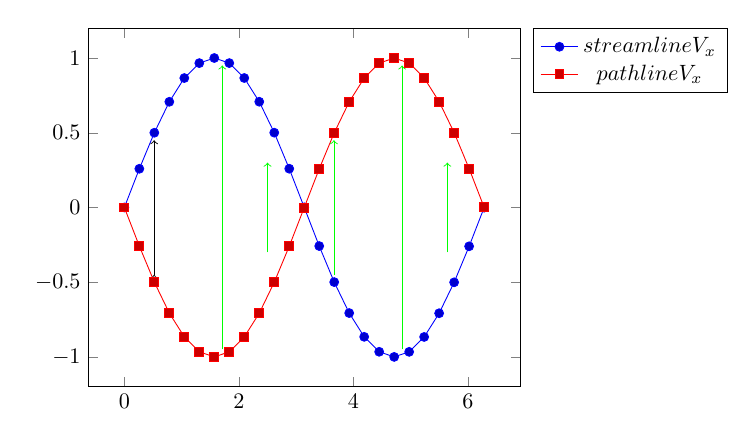
\begin{tikzpicture}[scale=0.8]
		\begin{axis}[domain=0:6.282,legend pos=outer north east]
        \addplot {sin(deg(x))}; 
        \addplot {-1*sin(deg(x))}; 
        \legend{$streamline V_{x}$,$pathline V_{x}$}
        \draw [->] (0.52,-0.45) edge (0.52,0.45);
        \draw [green, ->          ] (1.71,-0.95) -- (1.71,0.95);
        \draw [green, ->          ] (2.5,-0.3) -- (2.5,0.3);
        \draw [green, ->          ] (3.66,-0.45) -- (3.66,0.45);
        \draw [green, ->          ] (4.85,-0.95) -- (4.85,0.95);
        \draw [green, ->          ] (5.64,-0.3) -- (5.64,0.3);
		\end{axis}
		\end{tikzpicture}	
		\caption{$V_{x}$ of streamline and path line in Example two}
		\label{SPDFailStramAndPathX}
	\end{subfigure}
	\begin{subfigure}{0.5\textwidth}
		\centering
		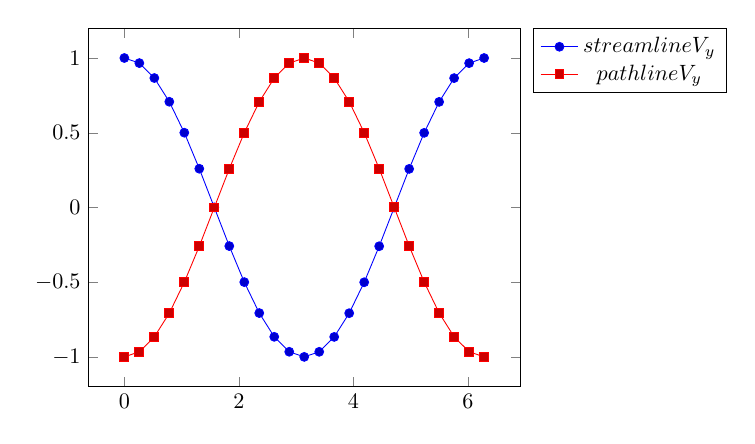
\begin{tikzpicture}[scale=0.8]
	    	\begin{axis}[domain=0:6.282,legend pos=outer north east]
			\addplot {cos(deg(x))}; 
			\addplot {-1*cos(deg(x))}; 
			\legend{$streamline V_{y}$,$pathline V_{y}$}
			\end{axis}
			\end{tikzpicture}	
			\caption{$V_{y}$ of streamline and path line in Example two}
			\label{SPDFailStramAndPathY}
		\end{subfigure}
	\caption{Those three picture show in the monotonous increasing case, how $SPD_{t_{n}}$ integrate $\Delta V$. As the $\Delta V\tau$  changed the sign, from positive to negative, which leads the integration result goes to zero when time=$2\pi$.}
	\label{fig:SPDFailWithVelocity}
\end{figure} 

Figure \ref{fig:SPDStreamPathlineWithVelocity} and figure \ref{fig:SPDFailWithVelocity} present the reason $SPD_{t_{n}}$ imprecise for measuring time-dependency when $\Delta V_{tau}$ has opposite direction. Therefore, in the next part of this Chapter, I will introduce another concept which develops from $SPD_{t}$.
\subsection{Definition}
Unlike $SPD_{t_{n}}$ only pays attention on the end point distance of streamline and path line, the follow concept, called \textbf{Sum Distance Difference of Streamline and Pathline} and marked as $SumDisDiff$, cares about all $SPD_{t},t\in[0,t_{n}]$.\\
Firstly, define the concept of \textbf{Distance Difference of streamline and path line between time $\tau$ and time $\chi$}, marked as $DisDiff(\vect{X}_{0},T,\chi,\tau)$, for short $DisDiff_{\chi}^{\tau}$. 
\begin{mydef}
	Distance Difference of streamline and path line between time $\tau$ and time $\chi$ is the absolute value of $SPD(\vect{X}_{0},T,\chi)$ and $(\vect{X}_{0},T,\tau)$ difference. Where both $\chi$ and $\tau$ are $\in [0,t_{n}]$.
\end{mydef}

Three special cases:\\
\begin{itemize}
	\item Distance Difference of streamline and path line between time 0 and time $t_{n}$ is equal to end point distance of streamline and path line.
	$$DisDiff(\vect{X}_{0},T,0,t_{n})=SPD(\vect{X}_{0},T,t_{n})$$
	\item If $\chi$ and $\tau$ are close to each other enough, i.e $\chi=\tau+ \varepsilon$, $\varepsilon\rightarrow 0$\\
	$$DisDiff(\vect{X}_{0},T,\chi,\tau)=0$$
	\item If divide time period $[0,t_{n}]$ into $t_{0}=0, t_{1},...,t_{i},...,t_{n}$, $DisDiff(\vect{X}_{0},T,t_{i},t_{i-1})$ , called neighbor distance differ, marked as $DisDiff_{t_{i}}$. In the figure \ref{fig:DisDiff}, green lines present $DisDiff_{t_{i}}$.\\
\end{itemize}

\begin{figure}[H]
	\centering
	\includegraphics[width=0.6\textwidth]{pic/tu3.pdf}
	\caption{{\tiny $DisDiff_{t_{i}}$. along the pathline and streamline.}}
	\label{fig:DisDiff}
\end{figure}

Mathematically, define $DisDiff(\vect{X}_{0},T,\chi,\tau), \tau>\chi$:\\
\begin{eqnarray}
DisDiff(\vect{X}_{0},T,\chi,\tau)=\biggr\lvert SPDis(\vect{X}_{0},T,\tau)-SPDis(\vect{X}_{0},T,\chi)\biggr\rvert\\
=\biggr\lVert\int_{t=\chi}^{t=\tau} (V(\phi^{t}(\vect{X}_{0}),T)-V(\psi^{t}(\vect{X}_{0}),T+t)) dt\biggr\rVert
\end{eqnarray}
For the special case three, neighbor distance differ is defined mathematically as below:\\
$$DisDiff_{t_{i}}=\biggr\lVert\int_{t=t_{i-1}}^{t=t_{i}} (V(\phi^{t}(\vect{X}_{0}),T)-V(\psi^{t}(\vect{X}_{0}),T+t)) dt\biggr\rVert$$
Moreover if $t_{i}=t_{i-1}+\varepsilon, \varepsilon\rightarrow 0$, then:\\
$$DisDiff_{t_{i}}=\int_{t=t_{i-1}}^{t=t_{i}} \lVert V(\phi^{t}(\vect{X}_{0}),T)-V(\psi^{t}(\vect{X}_{0}),T+t)\rVert dt$$
Along the streamline and path line, define \textit{Sum Neighbor Distance Differ}.
\begin{mydef}
Sum Neighbor Distance Differ along streamline and path line between time $0$ and time $t_{n}$ sums up all those $DisDiff_{t_{i}}, t_{i}\in[t_{0}, t_{n}]$, if divide time period $[0, t]$ into $t_{0}=0, t_{1},...,t_{i},...,t_{n}, \Delta t_{i}=t_{i}-t_{i-1}>0$, mark it as $SumDisDiff(\vect{X}_{0},T,t_{n})$
\end{mydef}

Mathematically, in discrete case, $SumDisDiff(\vect{X}_{0},T,t_{n})$ can be written as:
\\
$$SumDisDiff(\vect{X}_{0},T,t_{n})=\sum_{i=1}^{i=n}\lVert V(\phi^{t^{i}}(\vect{X}_{0},T),T)-V(\phi^{t^{i-1}}(\vect{X}_{0},T),T)+$$
$$V(\psi^{t_{i}}(\vect{X}_{0},T),T+t_{i})-V(\psi^{t_{i-1}}(\vect{X}_{0},T),T+t_{i-1})\rVert\cdot \Delta t_{i}$$
\\
if $t_{i}=t_{i-1}+\varepsilon, \varepsilon\rightarrow 0$, then the continuity case as below:
\begin{eqnarray}\label{Equation:SumDisDiff}
SumDisDiff(\vect{X}_{0},T,t_{n})=\int_{\tau=0}^{\tau=t_{n}} \lVert V(\phi^{\tau}(\vect{X}_{0}),T)-V(\psi^{\tau}(\vect{X}_{0}),T+\tau)\rVert d\tau
\end{eqnarray}
\subsection{Theorem}
According to the equation \ref{Equation:SumDisDiff}, unlike $SPD(\vect{X}_{0},T,t_{n})$, $SumDisDiff(\vect{X}_{0},T,t_{n})$ sums up the magnitude of the velocity changing at any moment along streamline and path line. Intuitively, in $SumDisDiff(\vect{X}_{0},T,t_{n})$ every change matters, no matter it is negative or positive. Therefore, even $SPD(\vect{X}_{0},T,t), t\in[0,t_{n}]$ is not monotonous, $SumDisDiff(\vect{X}_{0},T,t_{n})$ can weight time-dependency more accurate, which indicates that $SumDisDiff(\vect{X}_{0},T,t_{n})$ will not underestimate time-dependency property.\\
Especially, if $SPD(\vect{X}_{0},T,t), t\in[0,t_{n}]$ is monotonous increasing, then $SPD(\vect{X}_{0},T,t_{n})=SumDisDiff(\vect{X}_{0},T,t_{n})$, which means $SumDisDiff(\vect{X}_{0},T,t_{n})$ has better property to weight time-dependency for vector field data.
\begin{mytheory}
	Apply $SumDisDiff(\vect{X}_{0},T,t_{n})$ to visual time-dependency of vector field data set along stream lines and path lines. In those two cases mentioned, $SumDisDiff(\vect{X}_{0},T,t_{n})$ is greater, the vector data along stream line and path line is more strongly time-dependent. 
\end{mytheory}

\subsection{Result Comparison}
Below is the implement of computing $SumDisDiff(\vect{X}_{0},T,t_{n})$.\\
\begin{algorithm}[H]
	\KwData{Vector field data set}
	\KwResult{2D $SumDisDiff(\vect{X}_{0},T,t_{n})$ scalar field data}
	Set the time slice where streamlines and path line start.\\
	Select space area which seeds from and the number of seeds$s$.\\
	Get seeds by picking points uniform from the area.\\ 
	Set time step $\Delta t$ and time period $t_{n}$. \\
	Get number of points along one stream line and path line $n=\frac{t_{n}}{\Delta t}$.\\
	\For {$i\leftarrow 0$ \KwTo $s-1$}
	{
		Set seed coordinate $S_{i0}$\\
		Initial $SumDisDiff=0$
		\For{$j\leftarrow 0$ \KwTo $n-1$}{
			Get velocity $V_{ij}^{s}$ of the seed by Runge-Kutta 4th order interplation for streamline.\\
			Computing the next point $S_{ij+1}$ coordinate by $S_{ij}+V\cdot \Delta t$ of streamline;\\
			Get velocity $V_{ij}^{p}$ of the seed by Runge-Kutta 4th order interplation for path line.\\
			Computing the next point $P_{ij+1}$ coordinate by $P_{ij}+V\cdot \Delta t$ of path line;\\			
			Computing the $DisDiff=\lVert S_{ij+1}-P_{ij+1}\rVert$
			$SumDisDiff+=DisDiff$
		}
		Write $SumDisDiff$ to the seed position in the space.
	}
\end{algorithm}

Apply the algorithm on the data set mentioned before, and compare the result to the result of $SPD(\vect{X}_{0},T,t_{n})$ mentioned in \ref{fig:SPDResult}, so that the difference between those two concepts will be presented intuitively. Moreover, it is also significant to inspect the streamline and path line at the area where there exist different results.

\begin{figure}[H]
	\centering
	\begin{subfigure}{0.65\textwidth}
		\centering
		\includegraphics[width=0.75\textwidth]{pic/DisDiffResultST200Go60.png}
		\caption{$SumDisDiff(\vect{X}_{0},T,t_{n})$ where $T=5s, t_{n}=1.5s $. The area in the cycle is most different area compare to $SPD_{t_{n}}$ in the space.  }
	\end{subfigure}
	\begin{subfigure}{0.45\textwidth}
		\centering
		\includegraphics[width=0.65\textwidth]{pic/DiffDisAndSPDDifferentPathline.png}
		\caption{Choose a seed sample $\vec{X_{0}}(0.04,0.065)$  as an example where  $SumDisDiff$ is much greater than $SPD$, the picture shows the streamline and path line in the whole period 1.5s. }
	\end{subfigure}	
	\begin{subfigure}{0.45\textwidth}
			\centering
			\includegraphics[width=0.65\textwidth]{pic/DiffDisAndSPDDifferentPathlineMiddle6dot2s.png}
			\caption{The same seed as picture (b), but $t_{n}$ is 1.2s, and here shows the $SPD_{t=1.2s}$ actually is the maximum in the period 1.5s, i.e $SPD_{t}, t\in[0, 1.5s]$ is not monotonous}
	\end{subfigure}		
	\begin{subfigure}{0.55\textwidth}
			\centering
			\includegraphics[width=0.65\textwidth]{pic/DiffDisAndSPDDifferentPathlineMSameResult.png}
			\caption{Choose the seed $\vec{X_{0}}(0.024,0.06)$ as an example, where the result of $SPD$ and $DisDiff$ are almost equal. From the streamline and path line, the $SPD$ reaches to the maximum coincidentally, if extend $t_{n}$, then $SPD$ will decrease.}
	\end{subfigure}	
	\caption{Result of $SumDisDiff$ and comparison to $SPD$}
	\label{fig:ResultofSumDisDiff}			
\end{figure}
From figure \ref{fig:ResultofSumDisDiff}, except main different part of two result, the another mostly difference is the result of $DisDiff$ is much smoother than the result of $SPD$, as $DisDiff$ eliminates the "random property" of the $SPD$. This is presented clearer when compare the result of same seeds with different start time $T$ as below:
\begin{figure}[H]
	\centering
	\begin{subfigure}{0.45\textwidth}
		\centering
		\includegraphics[width=1\textwidth]{pic/SPDResulttime=5sgo1dot5sYnormal[5to2dot5s].png}
		\caption{ $SPD(\vect{X}_{0},T,t_{n})$ result, $T\in[5s,7.5s]$,$t_{n}=1.5s$ of all points $x_{0}=0.05,y\in[0,0.1]$, every column in the picture is the result of the seed at different T.}
	\end{subfigure}
	\begin{subfigure}{0.45\textwidth}
		\centering
		\includegraphics[width=1\textwidth]{pic/DisDiffResultY.png}
		\caption{$DisDiff(\vect{X}_{0},T,t_{n})$ result, $T\in[5s,7.5s]$,$t_{n}=1.5s$ of all points $x_{0}=0.05,y\in[0,0.1]$, every column in the picture is the result of the seed at different T. }
	\end{subfigure}	
		\label{fig:ResultofSumDisDiffY}			
\end{figure}	

\subsection{Average of $DisDiff_{t_{n}}$}
From equation \ref{Equation:SumDisDiff}, it is obvious that if hold $X_{0}$ and $T$, $SumDisDiff_{t_{n}}$ is monotonous increasing with $t_{n}$. Thence, comparing $SumDisDiff_{t_{n}}$ and $SumDisDiff_{t_{m}}$, where $t_{m}\neq t_{n}$ gives no so much information to judge the time-dependency property between two different time periods.\\
Therefor, define \textbf{$AverDisDiff(\vect{X}_{0},T,t_{n})$}, which is $SumDisDiff(\vect{X}_{0},T,t_{n})$ divide by $t_{n}$.
\begin{eqnarray}\label{Equation:AverDisdiff}
	AverDisDiff(\vect{X}_{0},T,t_{n})=\frac{\int_{\tau=0}^{\tau=t_{n}} \lVert V(\phi^{\tau}(\vect{X}_{0}),T)-V(\psi^{\tau}(\vect{X}_{0}),T+\tau)\rVert d\tau}{t_{n}}
\end{eqnarray}

\begin{figure}[H]
	\centering
	\begin{subfigure}{0.45\textwidth}
	   \centering
	   \includegraphics[width=0.65\textwidth]{pic/Averdiffdisstart250go50.png}
	   \caption{ The result of $AverDisDiff_{\tau=1.25s}$. Seeds start at time T= 6.25s go through 1.25s.}
	\end{subfigure}	
	\begin{subfigure}{0.45\textwidth}
	    \centering
		\includegraphics[width=0.65\textwidth]{pic/Averdiffdisstart250go80.png}
		\caption{ The result of $AverDisDiff_{\tau=2s}$. Seeds start at time T= 6.25s go through 2s.}
	\end{subfigure}	
	\caption{Comparing those pictures, it is easy to find out that time dependency of two data sets is similar with little difference, for instance the area at up-left is much smoother in the left figure.}
	\label{fig:AverDisDiffResult}
\end{figure}	
\subsection{Differential of $SumDisDiff$}//should give more detail
So far, no matter $SPD$ or $SumDisDiff$, both of them are presenting how much velocity change along the streamline and path line. Here we try to find out the path where acceleration change fast. Thence, for every seed in the space calculate the $SumDisDiff$ differential on start time $T$.
$$\frac{d SumDisDiff(\vect{X}_{0},T,t_{n})}{d T}$$ And highlight the path in the space for showing the highest acceleration area.
 \begin{figure}[H]
 	\centering
 	\begin{subfigure}{0.45\textwidth}
 		\centering
 		\includegraphics[width=0.65\textwidth]{pic/DiffertialOntime.png}
 		\caption{ The result of $SumDisDiff$ differential on time $T$ in the 2D space, it shows in the moment $T=5s$ and $t_{n}=1.5s$, along the streamline and path line, the red line area has great acceleration}
 	\end{subfigure}	
 	\begin{subfigure}{0.45\textwidth}
 		\centering
 		\includegraphics[width=0.65\textwidth]{pic/DiffertialOntimeY.png}
 		\caption{ The result of $SumDisDiff$ differential on time $T$ in the seeds $\vect{X_{0}}(x_{0},y_{0})$, where $ x_{0}=0.05, y_{0}\in[0,0.1] $, it shows the the acceleration changes}
 	\end{subfigure}	
 	\caption{All those path in those two pictures presenting the area $SumDisDiff$ changing fastest, which indicate velocity exists big difference along the streamlines and path lines from seeds $\xi(X_{0},T)$  }
 	\label{fig:SumDisDiffDifferetialResult}
 \end{figure}

\section{Exponential Regression of Sum Distance Difference of Streamlines And Path lines}\label{sec:Exponent}
In section \ref{sec:Distance}, $SPD$ fail to weight time-dependency of vector field, when $SPD_{t}, t\in[0,t_{n}]$ is not monotonous with time $t$. In section \ref{sec:SumDisDiff}, $SumDisDiff$ is a concept developed basing on $SPD$, which is always monotonous  with $t, t\in[0,t_{n}]$ and this property leads $SumDisDiff$ can be applied to weight time-dependency of different kinds of vector field data set.\\
\begin{figure}[H]
	\centering
	\begin{subfigure}{0.45\textwidth}
		\centering
		\includegraphics[width=0.65\textwidth]{pic/SumDisDiffAndSPD.png}
		\caption{ $SumDisDiff$ (blue) and $SPD$ (green) at seed $\vect{X_{0}}(0.049, 0.028)$, $T=6.25s$, $t_{n}=2s$.}
	\end{subfigure}
	\begin{subfigure}{0.45\textwidth}
		\centering
		\includegraphics[width=0.65\textwidth]{pic/streamlineandpathlinex=49y=28from250go2sExponetcase.png}
		\caption{ Streamline and path line from seed $\vect{X_{0}}(0.049, 0.028)$, $T=6.25s$, $t_{n}=2s$.}
	\end{subfigure}
	\begin{subfigure}{0.45\textwidth}
		\centering
		\includegraphics[width=0.65\textwidth]{pic/SumDisDiffAndSPD2.png}
		\caption{ $SumDisDiff$ (blue) and $SPD$ (green) at seed $\vect{X_{0}}(0.049, 0.020)$, $T=6.25s$, $t_{n}=2s$.}
	\end{subfigure}
	\begin{subfigure}{0.45\textwidth}
		\centering
		\includegraphics[width=0.65\textwidth]{pic/streamlineandpathlinex=49y=20from250go2sExponetcase.png}
		\caption{ streamline and path line from seed $\vect{X_{0}}(0.049, 0.028)$, $T=6.25s$, $t_{n}=2s$}
	\end{subfigure}
	
	\caption{Figure (a) and (c) show the $SumDisDiff$ and $SPD$ change in the time period $[0,2]$. figure (a) shows the case $SPD$ decreases during the later half part of time period, while figure (b) shows the $SPD$ almost keep monotonous increasing case. Figure (b) and (d) show streamlines and path lines in those two cases.}
	\label{fig:SPDandSumDisDiffCompare}
\end{figure}

In chapter: \ref{sec:SumDisDiff}, the time-dependency property of vector field data set is weighted by $SumDisDiff$ which sums up $DisDiff_{\tau}, \tau\in[0,t_{n}]$ and if $DisDiff_{\tau}$ is negative , use $-1\cdot DisDiff_{t}$ instead. In this chapter,  we introduce another concept called \textbf{Exponent of Regression}, marked as $\lambda$, which is developed basing on $SPD$ and $SumDisDiff$.
\subsection{Definition}
\begin{mydef}\label{Def:Exponent}
	Given a time period $[0,t_{n}]$, a seed $\xi(X_{0},T)$,pick $n$ moments in the time period uniformly $t_{0}=0,t_{1},t_{2},...,t_{i},...,t_{n-1},t_{n}$ and the set of those moments called \textbf{Sample Moment Set} $\Theta$, computing all $SPD_{\tau}$ and $SumDisDiff_{\tau}$, $\tau\in\Theta$. Take those $SumDisDiff_{\tau}$ as data samples, do exponent regression on time $t\in[0, t_{n}]$, where the regression model is:
	$$f(t)=\lambda e^{t}-\lambda$$
	Call $\lambda$ here \textbf{Exponent of Regression}.  $\lambda$ depends on $\xi(X_{0},T)$ and $t_{n}$.
\end{mydef}

Even $SumDisDiff$ integrates all velocity change along the path line and streamline, it still depends on $t_{n}$, which denotes different $t_{n}$ leads different $SumDisDiff$. Meanwhile, in Chapter \ref{sec:SumDisDiff}, $AverDisDiff$ can be used to compare time-dependency property of different end time, but it is just $\frac{SumDisDiff_{t_{n}}}{t_{n}}$, which may lead bigger mistake. For sure, linear regression or logarithm regression can be also applied here. However, the exponential regression feeds better result back.\\
\subsubsection{Exponential Regression And Least Square}
An exponential regression is the process of finding the equation of the exponential function that fits best for a set of data. It is one of the simplest nonlinear model, which usually is shown as below:
$$y_{i}=\beta_{0}+\beta_{1}\exp(\beta_{2}x_{i})+\epsilon_{i}$$
Where the $\epsilon_{i}$ are the independent and identically distributed normal with mean 0 and constance variance $\sigma^{2}$. Base on the model and data set, apply one kind of estimating methods to get estimated 
$\hat{\beta_{0}}$, $\hat{\beta_{1}}$ and $\hat{\beta_{2}}$ and call the difference between real value $y_{i}$ and estimated value $\hat{y_{i}}=\hat{\beta_{0}}+\hat{\beta_{1}}\exp(\hat{\beta_{2}}x_{i})$ residual.\\
In our case, $y_{i}$ in the model is the $SumDisDiff$ at moment $t_{i}$ and $x_{i}$ is time $t_{i}$.\\
The data for regression is sampled as described in the definition \ref{Def:Exponent}. As during the time period, $SumDisDiff$ always begins with 0. Therefore, adjust the original exponential regression model as below:\\ 
$$y_{i}=\lambda e^{t_{i}}-\lambda$$ where $i\in [1,n]$.\\
Then apply least squares method to get estimated $\hat{\lambda}$. The method of least squares is a standard approach in regression analysis to the approximate solution of overdetermined systems, i.e., sets of equations in which there are more equations than unknowns. "Least squares" means that the overall solution minimizes the sum of the squares of the residuals made in the results of every single equation.\\
Set the goal function $F(\lambda)$:
$$F(\lambda)=\sum_{i=1}^{i=n}(\lambda e^{t_{i}}-\lambda_{i}-SumDisDiff_{t_{i}})^{2}$$
And then $$\min_{\lambda} F(\lambda)$$
Differential on $\lambda$
$$F^{'}(\lambda)=\sum_{i=1}^{i=n}2(\lambda e^{t_{i}}-\lambda-SumDisDiff_{t_{i}})(e^{\lambda}-1)$$
Let $F^{'}(\lambda)=0$.\\
And get the estimated $\hat{\lambda}$:
\begin{eqnarray}
\label{Equation:lambda}
\hat{\lambda}=\frac{\sum_{i=1}^{i=n}SumDisDiff_{i}(e^{t_{i}}-1)}{\sum_{i=1}^{i=n}(e^{t_{i}}-1)}
\end{eqnarray}
Call the $\hat{\lambda}$ \textbf{Increasing Exponent of Time Dependency}.\\
Still take those two seeds mentioned before seed $\xi_{1}(X_{01}(49,28),T=6.25)$ and $\xi_{2}(X_{02}(49,20),T=6.25)$.
\begin{figure}[H]
	\centering
	\includegraphics[width=0.65\textwidth]{pic/EXponentRegressionOfSumDisDiff.png}
	\caption{ Blue points plot is the $SumDisDiff_{t}$ of seeds $x_{0}=0.049, y_{0}=0.028$ and blue line plot is the exponential regression of it and the $\hat{\lambda}=0.0162714$, while green points plot is the $SumDisDiff_{t}$ of seeds $x_{0}=0.049, y_{0}=0.020$ and green line plot is the exponential regression of it and the $\hat{\lambda}=0.0119348$}
	\label{fig:ExponentRegressionPlot}
\end{figure}
From the figure: \ref{fig:ExponentRegressionPlot}, it is easy to see the $\hat{\lambda}$ is greater the data is more strongly time-dependent along streamline and path line.\\
So far, the result seems reasonable, but it does not present obvious advantage compare to computing $SumDisDiff$, when it is used to compare time-dependency property between vectors along stream lines and path lines starting from different seed at the same time $T$ and $t_{n}$. Of course, it will be better to compare time-dependency property between streamlines and path lines with different $t_{n}$.
\begin{figure}[H]
	\centering
	\includegraphics[width=0.65\textwidth]{pic/ExponentRegressinlessTime.png}
	\caption{ Blue points plot is the $SumDisDiff_{t}$ of seeds $x_{0}=0.049, y_{0}=0.020$, $t_{n}=0.66s$ and blue line plot is the exponential regression of it and the $\hat{\lambda}=0.0306955$. Here the $\hat{\lambda}$ is even greater than the blue line in figure:\ref{fig:ExponentRegressionPlot}, which shows vector along the streamline and path line starting at seed  $x_{0}=0.049, y_{0}=0.020$ is strongly time dependency. At the same time, in the two period $t_{n}=2s , 0.66s$ between the two seeds, seeds $x_{0}=0.049, y_{0}=0.020$ shows more strongly time dependent generally. }
	\label{fig:ExponentRegressinlessTime}
\end{figure}
\subsection{Adjustment Increasing Exponent}
In the chapter \ref{sec:SumDisDiff}, the main difference between $SumDisDiff$ and $SPD$ is, when $SPD_{t}$ is not monotonous increasing, $SumDisDiff$ always adds up the positive value $DisDiff_{t}$ , but $SPD$ adds up positive and negative values, which depends on the direction of vector change. Consider about one simple case, two pairs of streamline and path line $SP_{a}$ and $SP_{b}$ starting at two different seeds $A$ and $B$ and end time $t_{n}=2s$. Suppose when $t\in[0,1]$, two sets of streamline and path line are exactly the same, while when $t\in[1,2]$, path line of $SP_{a}$ change the direction and go back to the seeds $A$  and path line of $SP_{b}$ goes the same direction as before. Basically, it is the case, $SumDisDiff$ plot during the time period is almost the same, but the $SPD$ plot during the period is quite different, which means one with fluctuation waves, one without. When we measure time-dependency property by $SumDisDiff$, those two cases are with the same time dependency property. However, the factor is those waves indicate strongly time-dependent, as the direction of vectors along the path line and streamline change leads to the wave.\\
//insert a picture or a gif to explain\\
\\
\\
\\
Therefore, here we introduce the concept of \textbf{Adjustment Increasing Exponent}, marked as $\hat{\lambda}^{+}$.
\begin{mydef}\label{Def:WaveDiff}
Given a time period $[0,t_{n}]$ and a seed $\xi(X_{0},T)$, pick $n$ moments in the time period uniformly $t_{0}=0,t_{1},t_{2},...,t_{i},...,t_{n-1},t_{n}$ and the set of those moments called \textbf{Sample Moment Set} $\Theta$, computing all $SPD_{\tau}$ and $SumDisDiff_{\tau}$, $\tau\in\Theta$.\\ 
Define \textbf{Wave Difference} as $SumDisDiff_{\tau}-SPD_{\tau}$, marked as $\omega_{\tau}$, take $\omega_{tau},\tau\in\Theta$  as data samples, do exponent regression on time $t\in[0, t_{n}]$, where the regression model is:
		$$f(t)=\lambda^{+} e^{t}-\lambda^{+}$$
Call $\lambda^{+}$ here \textbf{Adjustment Exponent of Regression}.  $\lambda^{+}$ depends on $\xi(X_{0},T)$ and $t_{n}$.
\end{mydef}
From the definition \ref{Def:WaveDiff}, the wave difference $\omega_{\tau}$ is always positive as $SumDisDiff_{\tau}$ is always greater than $SPD_{\tau}$. Moreover, $\omega_{\tau}, \tau\in[0,t_{n}]$ is almost monotonous which means:\\
if $\tau_{1}>\tau_{2}$, $\tau_{1},\tau_{2}\in[0,t_{n}]$\\
$$\omega_{\tau_{1}}>=\omega_{\tau_{2}}>=0$$
Special case, if $SPD_{\tau}, \tau\in[0,t_{n}]$ is monotonous increasing, $\omega_{\tau}=0$, $\forall \tau\in[0,t_{n}]$.
//insert a picture to show.\\
Still do exponential regression on  the time:\\
Set the goal function $F(\lambda^{+})$:
$$F(\lambda^{+})=\sum_{i=1}^{i=n}(\lambda e^{t_{i}}-\lambda_{i}-\omega_{t_{i}})^{2}$$
And then $$\min_{\lambda^{+}} F(\lambda^{+})$$
Differential on $\lambda^{+}$
$$F^{'}(\lambda^{+})=\sum_{i=1}^{i=n}2(\lambda^{+} e^{t_{i}}-\lambda^{+}-\omega_{t_{i}})(e^{\lambda^{+}}-1)$$
Let $F^{'}(\lambda^{+})=0$.\\
And get the estimated $\hat{\lambda}^{+}$:
\begin{eqnarray}
\label{Equation:lambda+}
\hat{\lambda}^{+}=\frac{\sum_{i=1}^{i=n}\omega_{i}(e^{t_{i}}-1)}{\sum_{i=1}^{i=n}(e^{t_{i}}-1)}
\end{eqnarray}
\begin{mydef}\label{Def:TrueLamda}
	In time-dependency analysis method, we call the result of $\hat{\lambda}+\hat{\lambda}^{+}$ \textbf{True Increasing Exponent of Time Dependency, mark it $\lambda$. } 
\end{mydef}
\begin{mytheory}\label{theo:tureincresingExponent}
	True Increasing Exponent can be used to measure time-dependency property along streamline and path line, and can be compared results of different end time $t_{n}$, different seed $\xi(X_{0},T)$, and the value is greater, the more strongly time-dependent is.
\end{mytheory}
\subsection{Result}

\begin{figure}[H]
	\centering
	\begin{subfigure}{0.3\textwidth}
		\centering
		\includegraphics[width=0.65\textwidth]{pic/LambdaSt250GO28.png}
		\caption{The $\hat{\lambda}(X_{0}, T=6.25, t_{n}=0.66)$ result.}
	\end{subfigure}
	\begin{subfigure}{0.3\textwidth}
		\centering
		\includegraphics[width=0.65\textwidth]{pic/AdjustLambdaSt250GO28.png}
		\caption{ The $\hat{\lambda}^{+}(X_{0}, T=6.25, t_{n}=0.66)$ result.}
	\end{subfigure}
	\begin{subfigure}{0.3\textwidth}
		\centering
		\includegraphics[width=0.65\textwidth]{pic/TotalLambdaSt250GO28.png}
		\caption{ The $\lambda(X_{0}, T=6.25, t_{n}=0.66)$ result.}
	\end{subfigure}
	
	\caption{The}
	\label{fig:lamadaResult0.66s}
\end{figure}

\begin{figure}[H]
	\centering
	\begin{subfigure}{0.3\textwidth}
		\centering
		\includegraphics[width=0.65\textwidth]{pic/LambdaSt250GO80.png}
		\caption{The $\hat{\lambda}(X_{0}, T=6.25, t_{n}=2)$ result.}
	\end{subfigure}
	\begin{subfigure}{0.3\textwidth}
		\centering
		\includegraphics[width=0.65\textwidth]{pic/AdjustLambdaSt250GO80.png}
		\caption{ The $\hat{\lambda}^{+}(X_{0}, T=6.25, t_{n}=2)$ result.}
	\end{subfigure}
	\begin{subfigure}{0.3\textwidth}
		\centering
		\includegraphics[width=0.65\textwidth]{pic/TotalLambdaSt250GO80.png}
		\caption{ The $\lambda(X_{0}, T=6.25, t_{n}=2)$ result.}
	\end{subfigure}
	
	\caption{}
	\label{fig:lamadaResult2s}
\end{figure}

\begin{figure}[H]
	\centering
	\begin{minipage}{0.45\textwidth}
		\centering
		\includegraphics[width=0.65\textwidth]{pic/SPDisStart250Go80.png}
		\caption{{\tiny SPDisStart250Go80 Green one $\lambda=0.00754665$, blue one $\lambda=0.0117781$}}
		\label{fig:SPDisStart250Go80}
	\end{minipage}
	\begin{minipage}{0.45\textwidth}
		\centering
		\includegraphics[width=0.65\textwidth]{pic/LamdaStart250Go80.png}
		\caption{{\tiny Lamda Start250 Go80}}
		\label{fig:LamdaStart250Go80}
	\end{minipage}
	
\end{figure}

We extract the main obvious difference part, can check how are streamlines and pathlines. 



\begin{figure}[H]
	\centering
	\begin{minipage}{0.45\textwidth}
		\centering
		\includegraphics[width=0.65\textwidth]{pic/streamlinepathlinex=30-40y=37Start250Go80.png}
		\caption{\tiny streamlinepathlinex=30-40y=37Start250Go80 }
		\label{fig:streamlinepathlinex=30-40y=37Start250Go80}
	\end{minipage}
	\begin{minipage}{0.45\textwidth}
		\centering
		\includegraphics[width=0.65\textwidth]{pic/SPDisPlotX=30,40Y=37Start250Go80.png}
		\caption{\tiny SPDisPlotX=30,40Y=37Start250Go80, Green one $\lambda=0.0171302$, blue one $\lambda=0.00887767$}
		\label{fig:SPDisPlotX=30,40Y=37Start250Go80}
	\end{minipage}
	
\end{figure}

\section{Time dependency analysis Given Fixed SPD or NorSPD}
In chapters before, all those algorithms mentioned are computing measurement basing on a fixed end time $t_{n}$, and then analyze time-dependency property of the vector along the streamline and path line in the time area $[0, t_{n}]$. Meanwhile, here offers another version to measure vector field time-dependency property by setting a fixed distance, which means set two massless particles, one follow the streamline and other one follow the path line, counting the time $t$ both of those two particles go until the distance between them reaching the value set, and mark the value $\mu$. Basing on the time $t$, analysis time dependency of the vector field.\\
As in some area the velocity is too small but still it is time dependency, then probably it would never reach the threshold set before. For avoiding this case, set fixed normalized distance of the end points of streamline and path line from the same seed just as defined in the chapter \ref{sec:Normal Distance}.\\
In this chapter, some ideas about \textbf{The Finite-Time Lyapunov Exponent(FTLE)},\textbf{ ridges}, \textbf{Lagrangian Coherent Structure(LCS)} will be mentioned. Actually, the idea of the algorithm to analyze time-dependency by given fixed $SPD$ or $NorSPD$ is inspired by the idea of FTLE. Therefore, at the beginning of this chapter, I will introduce theories about FTLE, ridge, and LCS.
\subsection{The Finite-Time Lyapunov Exponent}
As we described in chapter \ref{sec:DynamicSystem}, especially in unsteady flow dynamic system, the invariant manifolds helps people see how the system depends on time. The finite-time Lyapunov exponent(FTLE), which we will denote by $\sigma^{t}(X,T)$ is a scalar value which characterizes the amount of stretching about the trajectory of point $\xi(X,T)\in D$ over the time interval $[0, t]$> Here we can take the trajectory as path line. Actually, $\sigma^{t}(X,T)$ is the result after compare the stretching about trajectories of the point $\xi(X,T)\in D$  and points in neighbor, the amount of FTLE is greater, the trajectories separation is further.\\
\subsubsection{Definition}
To make the expression for the FTLE more specific, derive it from considering the stretching between two particles nearby:\\
\begin{center}
	$\xi_{1}(X,T)$ and $\xi_{2}(Y,T)$, where $Y=X+\delta X(0), \delta X\rightarrow 0$. \\
\end{center}
When those two particles flow after a while $t$, the new position:\\
\begin{center}
	$\psi^{t}(X,T)$ and $\psi^{t}(Y,T)$ 
\end{center}
Then measure the distance of $\psi^{t}(X,T)$ and $\psi^{t}(Y,T)$ .\\
$$\lVert\delta X(t)\rVert=\lVert\psi^{t}(X,T)-\psi^{t}(Y,T)\rVert$$
Taking the Taylor series expansion of the flow in point $\xi_{1}(X,T)$:\\
$$\psi^{t}(Y,T)=\psi^{t}(X+\delta X(0),T)=\psi^{t}(X,T)+\frac{d\psi^{t}(X,T)}{dX}\delta X(0)+O(\lVert\sigma X(0)\rVert^{2})$$
Then the distance of $\psi^{t}(X,T)$ and $\psi^{t}(Y,T)$ have the equation:\\
$$\lVert\delta X(t)\rVert =\biggr\rVert\frac{d\psi^{t}(X,T)}{dX}\delta X(0)+O(\lVert\sigma X(0)\rVert^{2})\biggr\lVert $$
Since $\delta X\rightarrow 0$, $O(\lVert\sigma X(0)\rVert^{2})$ is negligible limits to 0. Therefore, get the equation:\\

$\lVert\delta X(t)\rVert =\sqrt{\biggr\langle \frac{d\psi^{t}(X,T)}{dX}\delta X(0),\frac{d\psi^{t}(X,T)}{dX}\delta X(0) \biggr\rangle}$\\
$          =\sqrt{\biggr\langle \delta X(0),[\frac{d\psi^{t}(X,T)}{dX}]^{T}\cdot\frac{d\psi^{t}(X,T)}{dX}\delta X(0) \biggr\rangle}$
\\
Where $[\frac{d\psi^{t}(X,T)}{dX}]^{T}$ is the transpose of $\frac{d\psi^{t}(X,T)}{dX}$. And mark the symmetric matrix:\\
$$\vect{\Delta}(X,T,t)=[\frac{d\psi^{t}(X,T)}{dX}]^{T}\cdot\frac{d\psi^{t}(X,T)}{dX}\delta X(0)$$

When analysis time-dependency of flow, usually the maximum stretching or distance between $\psi^{t}(X,T)$ and $\psi^{t}(Y,T)$  would show the interesting time-dependency property of the vectors along those two trajectories, so that we try to find out the maximum distance:\\
$$\max_{\delta X(0)}\lVert\delta X(t)\rVert=\max_{\delta X(0)}\sqrt{\biggr\langle \delta X(0),\vect{\Delta}\delta X(0) \biggr\rangle}$$
And suppose $\lambda_{max}(\Delta)$ is the maximum value of the eigenvalue of the matrix $\vect{\Delta}$
and $\bar{\delta X(0)}$ is aligned with the eigenvector associated with $\lambda_{max}(\Delta)$, then we have :\\
$$\max_{\delta X(0)}\lVert\delta X(t)\rVert=\sqrt{\biggr\langle \bar{\delta X(0)},\lambda_{max}(\Delta)\bar{\delta X(0)\bar{\delta X(0)}} \biggr\rangle}=\sqrt{\lambda_{max}(\Delta)}\lVert\bar{\delta X(0)} \rVert$$
Now we define:\\
\begin{eqnarray}\label{Equation:FTLS}
  \sigma^{t}(X,T)=\frac{1}{T}ln\sqrt{\lambda_{max}(\Delta)}
\end{eqnarray}
and call the $\sigma^{t}(X,T)$ the finite-time Lyapunov exponent at the point $\xi(X,T)\in D$ with a finite integration time $t$. \\
Moreover, the maximum distance or stretching can be rewritten as:\\
$$\max_{\delta X(0)}\lVert\delta X(t)\rVert=\exp^{\sigma^{t}(X,T)\cdot T}\lVert\bar{\delta X(0)} \rVert$$
\subsubsection{Example}

\subsection{Ridge Surface and Iso Surface}

\subsection{Lagrangian Coherent Structure}



\subsection{LCS as Ridges in the FTLE Field}


Dynamical system, streamline, pathline and $SPDis$ are defined as we measure $SPDis$.\\
And this indicates that $SPDis$ is a accumulated and integrated value, usually some steps of big change leads $SPDis$ increasing fast.\\
As supposing the $V$ satisfies continuity, then:\\

The parameter $\mu$ is set to be the $SPDis$ the pathline and streamline would reach.\\
\begin{eqnarray}
\Gamma=\min_{t_{i}}\biggr(\biggr\lVert(\phi_{t_{0}}^{t_{i}}(\vect{X}_{0})-\psi_{t_{0}}^{t_{i}}(\vect{X}_{0})) \biggr\rVert>=\mu\biggr)
\end{eqnarray}
and call $\Gamma$ \textbf{Reach Time Exponent}.\\
Moreover, using $NorSPDis$ instead of $SPdis$.\\
\begin{eqnarray}
\zeta=\min_{t_{i}}\biggr(2\frac{\biggr\lVert(\phi_{t_{0}}^{t_{i}}(\vect{X}_{0})-\psi_{t_{0}}^{t_{i}}(\vect{X}_{0})) \biggr\rVert}{\sum_{t=t_{0}}^{t=t_{i}}[\lVert\phi_{t_{0}}^{t_{i}}(X_{0})-\phi_{t_{0}}^{t_{i-1}}(X_{0})\rVert+\lVert\psi_{t_{0}}^{t_{i}}(X_{0})-\psi_{t_{0}}^{t_{i-1}}(X_{0})\rVert]}>=\mu\biggr)
\end{eqnarray}

call $\zeta$ \textbf{Normalized Reach Time Exponent}

\subsection{Valley Surface Detection of Reach Time Exponent}
We can get a structured scalar field of Reach Time Exponent by computing $\Gamma$ at seed $X_{j}$ and $T_{i}$ and name the $\Gamma$, $\Gamma_{ij}$. As $X_{j}\in R^{2}$ and $_{i} \in R$, get a field $\Omega \subset R^{2}\times R$. Detect the valley surface of the structured scalar field, which shows the area which is most time dependency in the field.\\
Get the Hesse Matrix of the data and compare to get the surface.


\subsection{Entropy of Time Exponent}


Purpose\\
Real Time Exponent and Normalized Time Exponent show the time dependency of the area. However, how to measure if the time dependency characteristics is stable or predictable in a time range .
To analysis how velocity data changing during this time range, introduce the \textit{Entropy of time Exponent}.\\
Definition\\
Before defining the $Entropy$, it is necessary to get the sample of data. \\
Start streamlines and pathlines at $X_{0}$, but different times $T_{0}$ ,$T_{1}$ ,$T_{2}$ ...,$T_{i}$ ,...,$T_{n}$ in the dynamic system, and get $\Gamma_{0}$, $\Gamma_{1}$, $\Gamma_{2}$, ..., $\Gamma_{i}$, ..., $\Gamma_{n}$ for those different times.Suppose $\Delta T_{i}= T_{i}- T_{i-1}$, and for all $\Delta T_{i}$, $\Delta T_{i}=\Delta T$.
\begin{eqnarray}
Entropy=[1-\frac{1}{\log n}*\sum_{i=1}^{i=n}\frac{C_{i}}{C}*\log \frac{C_{i}}{C}]*\frac{\Gamma_{n}-\Gamma_{0}}{\frac{\sum{i=0}{i=n} \Gamma_{i}}{n}}
\end{eqnarray}
$n$ is the different times number\\
$$C_{i}=\left|\Gamma_{i+1}-\Gamma_{i}\right|$$
$$C=\sum\left|\Gamma_{j+1}-\Gamma_{j}\right|$$



\section{Sum And Average Distance of Streamline And Pathline}

	In some area, this case usually happens,i.e the value of $SPDis(\vect{X}_{0},t_{0},t_{n})$ is random in some level. For example, even $SPDis(\vect{X}_{0},t_{0},t_{n})$ is small, but it is possible that during time step $t_{0}$ to $t_{n}$, after some time  $_{m}$, $SPDis(\vect{X}_{0},t_{0},t_{m})$ is great which means data is very time dependency. For eliminating the random characteristics if $SPDis(\vect{X}_{0},t_{0},t_{n})$, we measure $Sum Distance of Streamline And Pathine (SumSPDis(\vect{X}_{0},t_{0},t_{n}))$ or  $Sum Normalized Distance of Streamline And Pathine (SumNorSPDis(\vect{X}_{0},t_{0},t_{n}))$.

	Generate a simple vortex data set, which keeps the core of vortex at the same point and the magnitude of $V$ keep increasing in the same $Delta V$.\\ 
	\begin{figure}[H]
		\centering
		\includegraphics[width=0.75\textwidth]{pic/SumData.png}
		\caption{{\tiny vortex data.}}
		\label{fig:SumVortexData}
	\end{figure}


	Exactly because the case in figure\ref{fig:SumSPDist=1s} and figure\ref{fig:SumSPDist=2s}, the $SPDis$ can be more casual because of the start seed and time. For example the $SPDis$ in figure\ref{fig:SumSPDist=1s} is much greater than in figure\ref{fig:SumSPDist=2s}, which is nonsense because the velocity in both of them have the same time dependency. So we define $SumSPDis$ and $AveSPDis$ to eliminate the randomly part of the $SPDis$. As the same reason as we mentioned in last section, we also define $SumNorSPDis$ and $AveNorSPDis$.\\
	\begin{itemize}
		\item $SumSPDis$
		$$SumSPDis(\vect{X}_{0},t_{0},t_{n})=\int_{t=t_{0}}^{t=t_{n}+t_{0}} SPDis(\vect{X}_{0},t_{0},t)dt$$
		\item $AveSPDis$
			$$AveSPDis(\vect{X}_{0},t_{0},t_{n})=\frac{1}{t_{n}}\int_{t=t_{0}}^{t=t_{n}+t_{0}} SPDis(\vect{X}_{0},t_{0},t)dt$$
		\item $SumNorSPDis$
		$$SumNorSPDis(\vect{X}_{0},t_{0},t_{n})=\int_{t=t_{0}}^{t=t_{n}+t_{0}} NorSPDis(\vect{X}_{0},t_{0},t)dt$$
		\item $AveNorSPDis$
				$$AveNorSPDis(\vect{X}_{0},t_{0},t_{n})=\frac{1}{t_{n}}\int_{t=t_{0}}^{t=t_{n}+t_{0}} NorSPDis(\vect{X}_{0},t_{0},t)dt$$
	\end{itemize}
	
	    \begin{figure}[H]
	    	\centering
	    	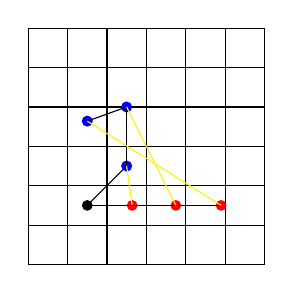
\begin{tikzpicture}[scale=0.50]
	    	\foreach \x in {1,2,...,6}
	    	\foreach \y in {1,...,6}
	    	{
	    		\draw (\x,\y) +(-.5,-.5) rectangle ++(.5,.5);
	    	}
	    	\node at (2,2) [fill,circle,scale=0.2] {$A$};
	    	\node at (3.14,2) [fill,circle,red,scale=0.2] {$A$};
	    	\node at (3,3) [fill,circle,blue,scale=0.2] {$B$};
	    	\node at (4.25,2) [fill,circle,red,scale=0.2] {$A$};
	    	\node at (3,4.5) [fill,circle,blue,scale=0.2] {$B$};
	    	\node at (5.4,2) [fill,circle,red,scale=0.2] {$A$};
	    	\node at (2,4.14) [fill,circle,blue,scale=0.2] {$B$};
	    	\draw (2,2)--(3,3);
	    	\draw (3,3)--(3,4.5);
	    	\draw (3,4.5)-- (2,4.14);
	    	\draw (2,2) .. controls (3.14,2) and (4.25,2) .. (5.4,2);
	    	\draw[yellow] (5.4,2)-- (2,4.14);
	    	\draw[yellow] (3,3)-- (3.14,2);
	    	\draw[yellow] (3,4.5)-- (4.25,2);
	    	\end{tikzpicture}
	    	\caption{\tiny black line with red points is the streamline at $t_{0}$, black line with blue points is the pathline starts at $t_{0}$, black point is the seed, and the lengths of yellow lines are the distance of end points of streamline and pathline $SPDis(X_{0},t_{1},t_{0})$,$SPDis(X_{0},t_{2},t_{0})$,$SPDis(X_{0},t_{3},t_{0})$, sum up those three length is the $SumSPDis$}
	    	\label{$SumSPDis$}
	    \end{figure}
	Apply $SumSPDis$ on the data set described before. Get the result as picture below shown:
			\begin{figure}[H]
				\centering
				\begin{minipage}{0.45\textwidth}
					\centering
					\includegraphics[width=0.45\textwidth]{pic/sumdisforsumdata.png}
					\caption{\tiny $SumSPDis$ of seeds at the time 0.25s and streamline and pathline go through 2.25s}
					\label{fig:sumdisforsumdata}
				\end{minipage}
				\begin{minipage}{0.45\textwidth}
					\centering
					\includegraphics[width=0.45\textwidth]{pic/disforsumdata.png}
					\caption{\tiny $SPDis$ of seeds at the time 0.25s and streamline and pathline go through 2.25s}
					\label{fig:disforsumdata}
				\end{minipage}
			\end{figure}
	Basing on the data information, time dependency of seeds with the same distance to the center. In figure\ref{fig:sumdisforsumdata}, we can see the case, while in figure\ref{fig:disforsumdata} this is not shown, as in some area the case in figure\ref{fig:SumSPDist=2s} happens.
	


	











\section{Analyze Time Dependency of the Whole Data}

 Purpose\\
	For detecting the time dependency characteristics of the whole data, and get the general idea of the whole data about time dependency characteristics. We introduce some parameters here.
 Definition \\
	\begin{itemize}
		\item Maximum (Minimum) Distance of Streamline And Pathline $MaxSPDis(\vect{X}_{0},t_{0},t_{n})$ and $MinSPDis(\vect{X}_{0},t_{0},t_{n})$:\\
		Computing the $SPDis(\vect{X}_{0},t_{0},t)$ from $ t_{0} $ to $t_{n}$ when construct the streamline and pathine, and pick the maximum and minimum.
		$$MaxSPDis(\vect{X}_{0},t_{0},t_{n})=\max_{t} SPDis(\vect{X}_{0},t_{0},t)$$
		$$MinSPDis(\vect{X}_{0},t_{0},t_{n})=\min_{t} SPDis(\vect{X}_{0},t_{0},t)$$
		\item Maximum (Minimum) Normalized Distance of Streamline And Pathline $MaxNorSPDis(\vect{X}_{0},t_{0},t_{n})$ and $MinNorSPDis(\vect{X}_{0},t_{0},t_{n})$:\\
		Computing the $NorSPDis(\vect{X}_{0},t_{0},t)$ at every time from $t_{0}$ to $t_{n}$ when construct the streamline and pathine, and pick the maximum and minimum.
		$$MaxNorSPDis(\vect{X}_{0},t_{0},t_{n})=\max_{t} NorSPDis(\vect{X}_{0},t_{0},t)$$
		$$MinNorSPDis(\vect{X}_{0},t_{0},t_{n})=\min_{t} NorSPDis(\vect{X}_{0},t_{0},t)$$
		\item Percentage of $SPDis(\vect{X}_{0},t_{0},t_{n})$ Smaller than Threshold $PerSPDis(\vect{X}_{0},t_{0},t_{n})$\\
		Set a parameter which is called \textit{distance threshold} $\mu$. Count the percentage of time when the $SPDis(\vect{X}_{0},t_{0},t)$  is less than the parameter.
		$$ PerSPDis(\vect{X}_{0},t_{0},t_{n})=\frac{\int_{t=t_{0}}^{t=t_{n}}(\mu-SPDis(\vect{X}_{0},t_{0},t)>0)}{t_{n}-t_{0}}$$
	\end{itemize} 
 Result Analysis\\
	\begin{tabular}{ l | l | l | l | l| l }
		Time Dependency& MaxSPdis & MinSPDis & MaxNorSPDis & MinNorSPDis & PerSPDid \\
		More & Great & Undefined & Great & Undefined & Small \\
		Less & Small & Small & Small& Small & Great\\
	\end{tabular}
\section{Distance of Streamlines Comparison}

 Purpose\\
	Computing $SPDis(\vect{X}_{0},t_{0},t_{n})$ or $NorSPDis(\vect{X}_{0},t_{0},t_{n})$ compares the streamline and pathline which shows time dependency characteristics of data during the time $[t_{0},t_{n}]$. However, in some case, for example during the time $[t_{0},t_{n}]$, the data in the start area ($X_{0}$ area) swings a lot i.e change to other state and change back, if the result we want to know is about the data change between two specific time. Then $SPDis(\vect{X}_{0},t_{0},t_{n})$ leads a big mistake, because perhaps as the data changed during the time, pathline goes to far away as pathine is a curve integrated.For example from one vortex to another vortex, then the pathline will go away from the area, but the streamline even at the end time will still at this area with a little change.\\ So here define streamline comparison.
	
	\begin{figure}[H]
			\centering
			\includegraphics[width=0.65\textwidth]{pic/streamlinecompareexample.png}
			\caption{streamlines at two moments are similar, but pathline go through those  two moments change a lot }
			\label{fig:streamlinecompareexample}
		\end{figure}
	\begin{figure}[H]
		\centering
		
		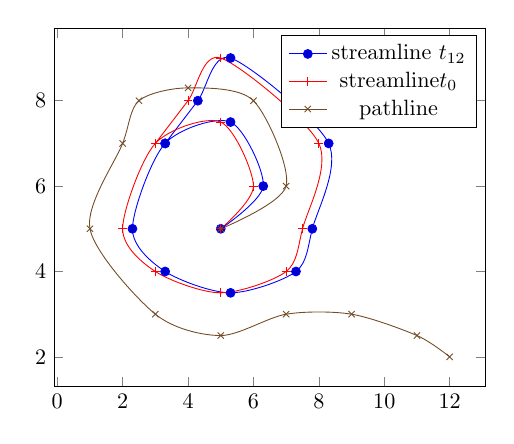
\begin{tikzpicture}[scale=0.8]
		
		\begin{axis}
		\addplot+[smooth,mark=*] plot coordinates
		{ (5,5) (6.3,6) (5.3,7.5) (3.3,7) (2.3,5) (3.3,4) (5.3,3.5) (7.3,4) (7.8,5) (8.3,7) (5.3,9) (4.3,8) (3.3,7) };
		\addlegendentry{streamline $t_{12}$ }
		
		\addplot+[smooth,mark=+] plot coordinates
		{ (5,5) (6,6) (5,7.5) (3,7) (2,5) (3,4) (5,3.5) (7,4) (7.5,5) (8,7) (5,9) (4,8) (3,7) };
		\addlegendentry{streamline$t_{0}$ }
		\addplot+[smooth,mark=x] plot coordinates
		{ (5,5) (7,6) (6,8) (4,8.3) (2.5,8) (2,7) (1,5) (3,3) (5,2.5) (7,3) (9,3) (11,2.5) (12,2)};
		\addlegendentry{pathline}
		\end{axis}
		\end{tikzpicture}
		
		\caption{Streamlines changed a little but pathine changed a lot}
		\label{when we use streamline to streamline}
	\end{figure}
 Definition\\
	$\phi_{t_{0}}^{t_{i}}(X_{0},T_{1})$ is the the point of the streamline at time $t_{i}$ start from $X_{0}$ at $T_{1}$.\\
	$\phi_{t_{0}}^{t_{i}}(X_{0},T_{2})$ is the the point in the streamline at time $t_{i}$ start from $X_{0}$ at $T_{2}$.\\
	Still we have in the dynamic system:\\
	\begin{eqnarray}
	\phi_{t_{0}}^{t_{m}+t_{n}}(\vect{X}_{0},T_{1})=\phi_{t_{m}+t_{0}}^{t_{n}}(\phi_{t_{0}}^{t_{m}}(\vect{X}_{0},T_{1}))=\phi_{t_{n}+t_{0}}^{t_{m}}(\phi_{t_{0}}^{t_{n}}(\vect{X}_{0},T_{1}))\\
	\phi_{t_{0}}^{t_{0}}(X_{0},T_{1})=X_{0}\\
	\phi_{t_{0}}^{t_{m}+t_{n}}(\vect{X}_{0},T_{2})=\phi_{t_{m}+t_{0}}^{t_{n}}(\phi_{t_{0}}^{t_{m}}(\vect{X}_{0},T_{2}))=\phi_{t_{n}+t_{0}}^{t_{m}}(\phi_{t_{0}}^{t_{n}}(\vect{X}_{0},T_{2}))\\
	\phi_{t_{0}}^{t_{0}}(X_{0},T_{2})=X_{0}\\
	\end{eqnarray}
	And define $Distance of Streamline (SSDis(\vect{X}_{0},t_{n},T_{1},T_{2}))$ as distance of points at time $t_{n}$ streamlines start at $X_{0}$ at $ T_{1} $ and $ T_{2} $.
	$$SSDis(\vect{X}_{0},t_{n},T_{1},T_{2})=\biggr\lVert \phi_{t_{0}}^{t_{i}}(X_{0},T_{1})-\phi_{t_{0}}^{t_{i}}(X_{0},T_{2})\biggr\rVert$$
	As similar as $NorSSdis(\vect{X}_{0},t_{n},T_{1},T_{2})$, define:
	$$NorSSDis(\vect{X}_{0},t_{n},T_{1},T_{2})=2*\frac{SSDis(\vect{X}_{0},t_{n},T_{1},T_{2})}{Slen(\vect{X}_{0},t_{n},T_{1})+Slen(\vect{X}_{0},t_{n},T_{2})}$$
	where $Sle1$ is length of streamline start $T$ along the curve.
	$$Slen(\vect{X}_{0},t_{n},T_{1},T)=\sum_{i=1}^{i=n}\biggr\lVert\phi_{t_{0}}^{t_{i}}(X_{0},T)-\phi_{t_{0}}^{t_{i-1}}(X_{0},T)\biggr\rVert$$
	where $t_{i}<=t_{n}$, and $t_{i}-t_{i-1}$ is the time step at $t_{i-1}$.













\begin{thebibliography}{9}	
	\bibitem{StreamlineDefine} 
	Definition of Streamlines
	\\\texttt{http://www.grc.nasa.gov/WWW/k-12/airplane/stream.html}
	
	\bibitem{PathlineDefine} 
	Definition of Pathlines
	\\\texttt{https://en.wikipedia.org/wiki/Streamlines,streaklines,andpathlines}
	
	\bibitem{DoublePendulum} 
	Picture of Double Pendulum Trajectory
	\\\texttt{https://en.wikipedia.org/wiki/Doublependulum}
	\bibitem{}

\end{thebibliography}









\end{document}